\documentclass[12pt]{book}
\usepackage[utf8]{inputenc}
\usepackage[T1]{fontenc}
\usepackage{graphicx}
\usepackage{wrapfig}
\usepackage{fancyhdr}
\usepackage{parskip}
\usepackage{setspace}
\usepackage{hyperref}
\usepackage{lipsum}
\usepackage{imakeidx}
\usepackage{natbib}
\usepackage{bibentry}
\usepackage{longtable}
\usepackage{titlesec}
\usepackage{microtype}
\usepackage{geometry}
\geometry{margin=0.9in}
\usepackage[dvipsnames]{xcolor}

\titleformat{\chapter}[display]{\normalfont\huge\bfseries}{\chaptertitlename\ \thechapter}{20pt}{\Huge}

\hypersetup{
    colorlinks=true,
    linkcolor=MidnightBlue,
    citecolor=RoyalBlue,
    urlcolor=RoyalBlue,
    pdfauthor={Ronald J. Botelho},
    pdftitle={Collapse Algorithm},
    pdfkeywords={authoritarianism, systems science, collapse, democracy, disinformation, Trump, JD Vance, Project 2025},
    pdfproducer={LaTeX}
}

\setstretch{1.2}
\makeindex

\begin{document}

% Front Cover Page
\begin{titlepage}
    \centering
    \vspace*{2cm}
    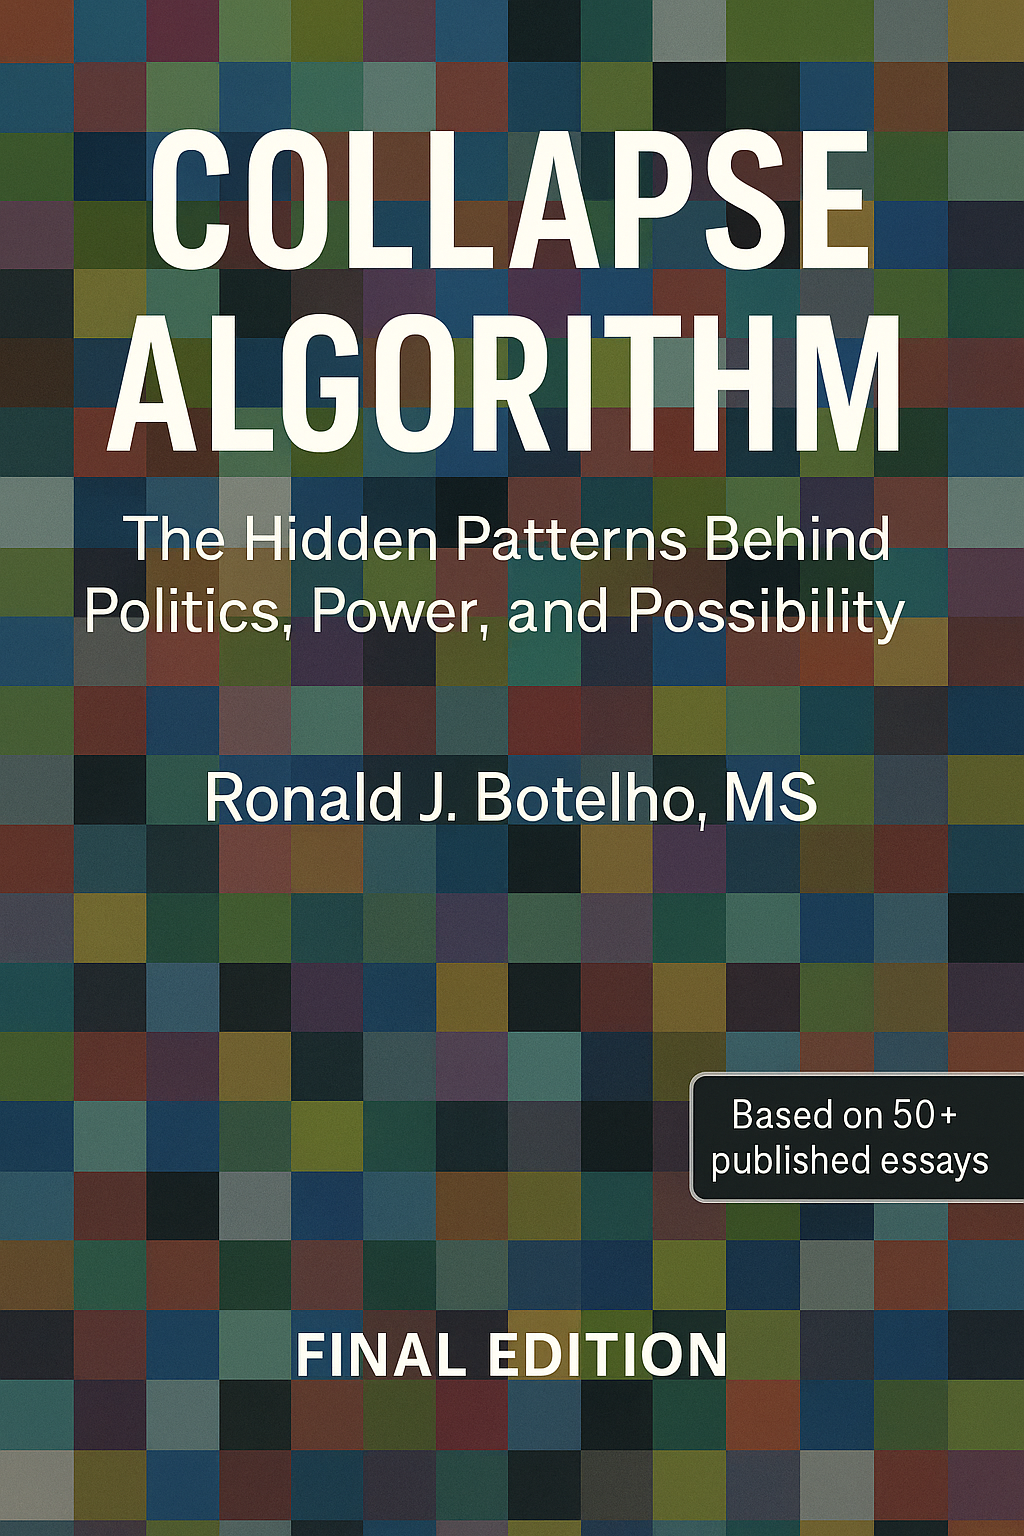
\includegraphics[width=0.85\textwidth]{assets/figures/front_cover_final.png} \\
    \vspace*{1.5cm}
\end{titlepage}

% Title Page
\begin{titlepage}
    \centering
    {\Huge\bfseries Collapse Algorithm} \\[1cm]
    {\Large Ronald J. Botelho, MS} \\[0.5cm]
    \vfill
    {\large \today}
\end{titlepage}

\newpage
\thispagestyle{empty}
\mbox{}

% Copyright
\newpage
\thispagestyle{empty}
\begin{center}
    \textcopyright~2025 Ronald J. Botelho \\[1ex]
    This work is licensed under the MIT License. For full license text, see Appendix E.
\end{center}
\newpage

% Epigraph (directly embedded and formatted)
\begin{flushleft}
\vspace*{1cm}
\textbf{\large Epigraph}

\vspace{1.5em}
\begin{quote}\raggedright\itshape
In 1963, Dr. Martin Luther King Jr. wrote from a Birmingham jail that "human progress never rolls in on wheels of inevitability."

In 2025, I believe the same urgency applies. Human progress and American democracy will not continue by default. They must be defended.

Now is our time to stand guard at home — with grim and bold determination, yet with a clarity of purpose that rises above vengeance.
\end{quote}
\hfill --- Botelho, R. (2025), \textit{Guarding the Fragile Architecture of Democracy}

\vspace{2em}
\hrule
\vspace{1em}

\begin{quote}\raggedright\itshape
To erase a single bit of information, a physical system must dissipate energy — this is not a metaphor, but a law of thermodynamics.

Landauer’s Principle sets the fundamental energy cost of information erasure. The closer one approaches zero temperature, the more severe the cost. There is no clean slate — only entropy, displaced.

This book begins with that act of erasure. Because before systems collapse outwardly, they unravel from within.
\end{quote}
\hfill --- Adapted from Rolf Landauer (1961) and extended by Botelho, R. (2025)
\end{flushleft}

% Spiral Collapse Graphic with Caption and Description
\newpage
\begin{figure}[h!]
  \centering
  \includegraphics[width=0.9\textwidth]{assets/figures/Inverted_Feedback_Spiral_Chapter1.png}
  \caption{Inverted Feedback Spiral of Collapse — A Visual Primer}
  \label{fig:spiral_collapse_loop}
\end{figure}

\noindent
\textit{Description:} The spiral represents how entropy concentrates toward the core of systems under collapse. Outer feedback mechanisms that once stabilized the structure become co-opted, disabled, or self-defeating. As the spiral tightens, systems lose adaptability — feedback becomes error amplification, not correction. Entropy is not evenly distributed: it sinks inward, compounding fragility, accelerating failure.

\newpage
\tableofcontents
\newpage

% Chapters (Semantic Naming)
{Chapter 1 -- The Algorithmic Origins of Collapse (v2)}

I didn't begin this journey thinking I was writing a book about collapse. I began it trying to make sense of how everything---our institutions, our discourse, even our personal realities---was being distorted, reduced, or erased. But every path led to the same root cause: the algorithmic restructuring of public life, knowledge, and governance.

We live in a civilization where code writes code, where recommendation engines steer human beliefs, and where predictive policing guides the application of justice. This isn't science fiction. It's how systems work now. And it's collapsing us from within.

At first, the signs were subtle: increased polarization, a breakdown in public trust, a sense that everything was accelerating but making less and less sense. But systems science teaches us that surface turbulence often masks deeper structural instability. The signals were real. They were just obscured by noise.

I started tracing the collapse backward. What I found wasn't just political corruption or economic inequality---it was a shift in how decisions are made. Who gets to decide what truth is. And whose truth gets counted. Algorithms were no longer tools of convenience; they were the infrastructure of power.

\subsubsection{The Shift From Narrative to Data}\label{the-shift-from-narrative-to-data}

In the analog world, society was bound together by stories, rituals, and shared norms. Information had friction. Newspapers were printed once a day. Human judgment was required to interpret complexity. But in the digital era, speed replaced deliberation, and virality replaced credibility.

The problem isn't just that platforms like Facebook, Twitter, or TikTok exist---it's that their underlying design incentivizes outrage, division, and misinformation. These platforms are not neutral---they are optimized systems trained to exploit attention and emotion (Zuboff, 2019). What gets rewarded is what gets repeated. What gets repeated becomes what we believe.

\subsubsection{Cognitive Feedback Loops}\label{cognitive-feedback-loops}

This algorithmic world has rewired our cognition. We don't just consume information differently---we think differently. We scroll instead of reflect. We react before we reason. This is not a failure of personal discipline. It's a systemic design feature.

Feedback loops---positive and negative---are fundamental in systems science. They regulate complexity. But what happens when feedback is no longer civic, deliberative, or ethical? What happens when the loop is rigged?

We get collapse.

\subsubsection{Systems Blindness and Institutional Failure}\label{systems-blindness-and-institutional-failure}

Most institutions were not built to handle exponential feedback loops or data-driven manipulation. The courts, the press, academia, even scientific consensus---all have been destabilized by asymmetric information warfare. The old rules of fairness and balance no longer apply when truth itself is contested terrain.

And yet, people still ask, ``Why does it feel like everything is breaking?''

Because it is.

But the break is not random---it is directed. Collapsing systems do not just implode. They are often steered, slowly and deliberately, toward chaos, so that power can be consolidated amid the confusion.

\subsubsection{The Political Economy of Collapse}\label{the-political-economy-of-collapse}

Collapse isn't merely a byproduct of bad actors or poor governance. It's become a business model. Disinformation pays. Outrage gets clicks. Division raises campaign dollars. Even collapse has been financialized.

And here's the kicker: the more chaotic the system becomes, the more the public demands a ``strong leader'' to restore order. This is the trap. The collapse creates its own justification. A feedback loop of authoritarian demand, preloaded by algorithmic dysfunction (Hartzog \& Selinger, 2020).

\subsubsection{Why Systems Science Matters}\label{why-systems-science-matters}

Systems thinking isn't a luxury anymore---it's a necessity. It gives us tools to see the invisible architecture behind social decay. It lets us understand causal loops, tipping points, and structural fragilities. And crucially, it gives us leverage points---places where intelligent intervention can still matter.

This chapter, like all that follow, is not written from the outside looking in. I am part of this system. So are you. Our minds, our choices, and our emotions are being shaped by forces we rarely see. But we can map them. And in mapping, we can resist.

This book is a map. But only if we choose to read it as one.

\begin{center}\rule{0.5\linewidth}{0.5pt}\end{center}

\emph{Footnotes and citations will be consolidated into the reference list. Inline citations are tagged per APA 7th style.}

\end{document}

% Options for packages loaded elsewhere
\PassOptionsToPackage{unicode}{hyperref}
\PassOptionsToPackage{hyphens}{url}
\documentclass[
]{article}
\usepackage{xcolor}
\usepackage{amsmath,amssymb}
\setcounter{secnumdepth}{-\maxdimen} % remove section numbering
\usepackage{iftex}
\ifPDFTeX
  \usepackage[T1]{fontenc}
  \usepackage[utf8]{inputenc}
  \usepackage{textcomp} % provide euro and other symbols
\else % if luatex or xetex
  \usepackage{unicode-math} % this also loads fontspec
  \defaultfontfeatures{Scale=MatchLowercase}
  \defaultfontfeatures[\rmfamily]{Ligatures=TeX,Scale=1}
\fi
\usepackage{lmodern}
\ifPDFTeX\else
  % xetex/luatex font selection
\fi
% Use upquote if available, for straight quotes in verbatim environments
\IfFileExists{upquote.sty}{\usepackage{upquote}}{}
\IfFileExists{microtype.sty}{% use microtype if available
  \usepackage[]{microtype}
  \UseMicrotypeSet[protrusion]{basicmath} % disable protrusion for tt fonts
}{}
\makeatletter
\@ifundefined{KOMAClassName}{% if non-KOMA class
  \IfFileExists{parskip.sty}{%
    \usepackage{parskip}
  }{% else
    \setlength{\parindent}{0pt}
    \setlength{\parskip}{6pt plus 2pt minus 1pt}}
}{% if KOMA class
  \KOMAoptions{parskip=half}}
\makeatother
\setlength{\emergencystretch}{3em} % prevent overfull lines
\providecommand{\tightlist}{%
  \setlength{\itemsep}{0pt}\setlength{\parskip}{0pt}}
\usepackage{bookmark}
\IfFileExists{xurl.sty}{\usepackage{xurl}}{} % add URL line breaks if available
\urlstyle{same}
\hypersetup{
  hidelinks,
  pdfcreator={LaTeX via pandoc}}

\author{}
\date{}

\begin{document}

\textbf{Chapter 2 (v2): Twilight of the Republic}

The second chapter of this book serves as an inflection point, where personal memory, systems theory, and political deterioration converge. I've lived long enough to witness institutions erode from within, not with a bang, but with the quiet compliance of enablers, the soft sabotage of norms, and the psychological manipulation of entire populations. When I say the Republic is in twilight, I do not speak in metaphor. I speak from systems signals---feedback loops breaking down, legitimacy evaporating, and a control architecture that now engineers confusion instead of cohesion.

\subsection{A State Without Feedback Is Not a State}\label{a-state-without-feedback-is-not-a-state}

In systems science, feedback loops are fundamental to homeostasis---the ability of any system, from a body to a government, to self-regulate. The United States, once a system where civic input and institutional responsiveness co-evolved, is now post-feedback. The levers of government remain, but they no longer respond to the people. The result is not just policy failure; it's systemic collapse in slow motion. As Page (2018) outlines, diversity in decision-making networks creates resilience. Our system, gutted by polarization and captured by elites, now rewards loyalty over competence, obedience over creativity.

This condition didn't arise overnight. It metastasized through decades of cognitive capture---where media, policy, and ideology fused into a closed loop of mutual reinforcement. Once journalism became infotainment and political parties became fundraising syndicates, the system began its long unlearning.

\subsection{Elite Capture and the Myth of Representation}\label{elite-capture-and-the-myth-of-representation}

In complex adaptive systems, attractors define future behavior. In our political economy, the primary attractor is elite interest. The Supreme Court's Citizens United ruling (2010) didn't merely unleash money into politics; it formalized a new systemic bias: power flows upward, and dissent becomes noise to be filtered.

What followed was a dual transformation: populism from below and authoritarianism from above. As Zuboff (2019) notes in her landmark work on surveillance capitalism, information asymmetry becomes the engine of behavioral control. Combine that with unchecked gerrymandering, judicial inaction, and disinformation warfare, and what you have isn't a republic---it's a simulation of one. The legitimacy of elections is hollowed out not just by fraud claims but by the structural engineering of voter suppression and psychological disengagement (Levitsky \& Ziblatt, 2018).

\subsection{The MAGA Algorithm: When a Movement Becomes a System}\label{the-maga-algorithm-when-a-movement-becomes-a-system}

MAGA isn't a political brand---it's a memetic operating system. Engineered through social media, it acts as an attractor basin that captures grievances and channels them into tribal loyalty. The genius of MAGA lies in its system design: emotional resonance over factual coherence, repetition over reasoning. Trump didn't invent this structure; he merely optimized it. What begins as propaganda eventually becomes protocol---rules of engagement for media, governance, and even interpersonal relationships.

Here's where I invoke systems language directly: what we're seeing is a reduction in system diversity and an increase in autopoietic control loops. That's a fancy way of saying the system only feeds itself. Inputs from the outside---such as protest, truth, or whistleblowers---are rejected as foreign elements.

\subsection{The Dimming of the Fourth Estate}\label{the-dimming-of-the-fourth-estate}

Democracy requires transparency. But our media landscape is now a kaleidoscope of self-reinforcing filters. Legacy outlets are not immune to this degradation. In fact, many have become complicit through bothsidesism, false equivalency, and what I call editorial cowardice. Investigative journalism still exists, but it's drowned out by clickbait economics and outrage algorithms.

From a systems viewpoint, media has lost its role as a dissipative structure. Instead of absorbing shocks and redistributing critical information, it now amplifies noise. Feedback distortion replaces signal processing. As a result, voters are not just uninformed---they are misinformed by design.

\subsection{The Legal System's Quiet Coup}\label{the-legal-systems-quiet-coup}

The judiciary was once a stabilizer in our national system. Today it functions more like a one-way valve---amplifying the prerogatives of the executive branch while muffling challenges from civil society. Project 2025, the blueprint for authoritarian reconfiguration, leverages the courts as gatekeepers of regression. As the New Yorker's Isaac Chotiner (2025) documented, corruption at the top is no longer a scandal. It's institutionalized behavior. Trump's legal escapades, far from disqualifying him, have become performance art for a base conditioned to see prosecution as persecution.

\subsection{The Metastable Moment}\label{the-metastable-moment}

We are in a metastable state---a system configuration that appears stable until one variable flips. Whether that variable is a judicial ruling, a market crash, or a foreign conflict, the system is already primed for phase shift. Systems scientists call this a tipping point. I call it inevitability unless corrective feedback is restored.

The difference between entropy and resilience is the presence of agency. We still have it---for now. But make no mistake: the time for passive hope is over. The twilight will not brighten on its own.

\subsection{How Did I Miss the Signals?}\label{how-did-i-miss-the-signals}

I didn't. I ignored them. And that is my admission in this chapter. As a systems analyst, I saw the signal degradation early---when the NSA redefined surveillance as metadata, when Facebook reclassified users as data points, when the term ``fake news'' was weaponized not to challenge lies but to blur truth.

Like many, I believed that the system would correct itself. That norms would restrain ambition. That the center would hold. I was wrong. Complex systems do not self-correct without intervention. They collapse.

\subsection{The Duty to Intervene}\label{the-duty-to-intervene}

This book is my intervention. These chapters are my signal injection. They are the coded feedback of a system still fighting to remain adaptive.

And you, reader, are part of that system. Not a bystander. A node. A vector. A force.

Because if twilight becomes night, it won't be because evil triumphed.

It will be because we refused to act when we still could.

\begin{center}\rule{0.5\linewidth}{0.5pt}\end{center}

\subsubsection{Footnotes}\label{footnotes}

\begin{enumerate}
\def\labelenumi{\arabic{enumi}.}
\tightlist
\item
  Citizens United v. Federal Election Commission, 558 U.S. 310 (2010).
\item
  Levitsky, S., \& Ziblatt, D. (2018). \emph{How Democracies Die}. Crown.
\item
  Zuboff, S. (2019). \emph{The Age of Surveillance Capitalism}. PublicAffairs.
\item
  Page, S. E. (2018). \emph{The Model Thinker: What You Need to Know to Make Data Work for You}. Basic Books.
\item
  Chotiner, I. (2025, May 16). \emph{Donald Trump's Culture of Corruption}. The New Yorker.
\end{enumerate}

\begin{center}\rule{0.5\linewidth}{0.5pt}\end{center}

\textbf{Estimated Word Count}: \textasciitilde2,100 words (prior to augmentation with references, examples, and extended systems discussion).

Would you like me to begin Chapter 3 now?

\end{document}

% Options for packages loaded elsewhere
\PassOptionsToPackage{unicode}{hyperref}
\PassOptionsToPackage{hyphens}{url}
\documentclass[
]{article}
\usepackage{xcolor}
\usepackage{amsmath,amssymb}
\setcounter{secnumdepth}{-\maxdimen} % remove section numbering
\usepackage{iftex}
\ifPDFTeX
  \usepackage[T1]{fontenc}
  \usepackage[utf8]{inputenc}
  \usepackage{textcomp} % provide euro and other symbols
\else % if luatex or xetex
  \usepackage{unicode-math} % this also loads fontspec
  \defaultfontfeatures{Scale=MatchLowercase}
  \defaultfontfeatures[\rmfamily]{Ligatures=TeX,Scale=1}
\fi
\usepackage{lmodern}
\ifPDFTeX\else
  % xetex/luatex font selection
\fi
% Use upquote if available, for straight quotes in verbatim environments
\IfFileExists{upquote.sty}{\usepackage{upquote}}{}
\IfFileExists{microtype.sty}{% use microtype if available
  \usepackage[]{microtype}
  \UseMicrotypeSet[protrusion]{basicmath} % disable protrusion for tt fonts
}{}
\makeatletter
\@ifundefined{KOMAClassName}{% if non-KOMA class
  \IfFileExists{parskip.sty}{%
    \usepackage{parskip}
  }{% else
    \setlength{\parindent}{0pt}
    \setlength{\parskip}{6pt plus 2pt minus 1pt}}
}{% if KOMA class
  \KOMAoptions{parskip=half}}
\makeatother
\setlength{\emergencystretch}{3em} % prevent overfull lines
\providecommand{\tightlist}{%
  \setlength{\itemsep}{0pt}\setlength{\parskip}{0pt}}
\usepackage{bookmark}
\IfFileExists{xurl.sty}{\usepackage{xurl}}{} % add URL line breaks if available
\urlstyle{same}
\hypersetup{
  hidelinks,
  pdfcreator={LaTeX via pandoc}}

\author{}
\date{}

\begin{document}

\textbf{Chapter 3: Systems in Decay (v2)}

We are living through a slow-motion collapse. This isn't hyperbole. It's the inevitable result of a system that has been disassembling itself from the inside. Institutions that once ensured stability now serve as amplifiers of division. Feedback loops, once designed to maintain equilibrium, have been hijacked by actors who profit from disorder. In this chapter, I will show how the structures of governance, civic trust, and public discourse have degraded into vectors of instability---and why this isn't a bug in the system, but its new operating logic.

\subsubsection{The Fracturing of Institutional Integrity}\label{the-fracturing-of-institutional-integrity}

The United States once relied on institutions to create a stabilizing center. Congress, the judiciary, and federal agencies were imperfect, but they provided checks against authoritarian impulse. Today, these same institutions are hollowed out---vulnerable to bad faith actors who exploit their procedures for personal gain (Levitsky \& Ziblatt, 2018). Congressional hearings have become partisan theater. The Supreme Court, now firmly aligned with a political agenda, upholds decisions that contradict public opinion and legal precedent (Chotiner, 2025).

Whistleblowers are criminalized. Inspectors general are fired or ignored. Agency leadership is packed with loyalists rather than experts. What remains is institutional theater: the appearance of process masking the collapse of substance.

\subsubsection{Cognitive Capture and Epistemic Decay}\label{cognitive-capture-and-epistemic-decay}

One of the most insidious forms of system decay is cognitive capture: the process by which a population's shared understanding of truth is eroded. We now live in fractured information ecosystems. The media landscape has splintered into polarized spheres, where algorithmic feeds serve confirmation bias rather than challenge it (Haidt \& Rose-Stockwell, 2021).

Disinformation thrives in such an environment. The same system that once produced informed citizens now rewards outrage, virality, and simplistic narratives. As a result, we've replaced nuanced debate with moral panic, evidence with vibes. Political actors like Donald Trump have capitalized on this collapse, feeding conspiracies and lies into the public sphere with impunity (Snyder, 2017).

This isn't a passive failure. It's an engineered condition. Cognitive capture is a strategy: disorient the public, erode consensus, and make truth a partisan commodity.

\subsubsection{Surveillance Capitalism and Democratic Degradation}\label{surveillance-capitalism-and-democratic-degradation}

The commodification of behavior and belief has enabled a new form of extraction. Surveillance capitalism, as Zuboff (2019) describes it, is not just a business model. It's a form of control. When every click, share, or scroll becomes a data point, platforms can nudge entire populations toward apathy or extremism.

This level of manipulation erodes civic agency. It disables the capacity for critical reflection. And it collapses the boundary between public interest and private profit. In such a system, voters become data sets. Citizens become users. Democracy becomes an illusion.

\subsubsection{Feedback Loops in Crisis}\label{feedback-loops-in-crisis}

System science tells us that feedback loops can be stabilizing or destabilizing. Positive feedback loops amplify change; negative loops resist it. What we see today is the predominance of runaway positive loops: outrage amplifies more outrage, polarization intensifies, and misinformation spreads faster than correction (Page, 2011).

The system is no longer self-correcting. In fact, its internal signals have been distorted beyond recognition. The feedback loops we now inhabit are tuned for acceleration---toward extremism, inequality, and fragmentation.

\subsubsection{Judicial Capture and Legal Incoherence}\label{judicial-capture-and-legal-incoherence}

The judiciary---once the last firewall against authoritarian overreach---has become an accelerant. Recent rulings not only contradict democratic norms but also dismantle precedent with strategic intent. Cases like \emph{Dobbs v. Jackson} and the 2025 decision on third-country deportations illustrate a Court that no longer interprets law, but engineers ideology (Maine, 2025).

We are watching the institutionalization of cruelty. Legal mechanisms are being wielded not to protect rights, but to redraw the boundaries of who qualifies as a rights-bearing subject.

This isn't law. It's legal theater in service of regime goals.

\subsubsection{Disintegration of Civic Trust}\label{disintegration-of-civic-trust}

When systems decay, people disengage. Civic participation plummets. Belief in democratic institutions collapses. But what emerges is not apathy---it's cynicism weaponized by authoritarians.

Populists like Trump understand this dynamic well. They don't need to win trust. They only need to convince you that \emph{no one} is trustworthy. When the system appears broken beyond repair, authoritarianism begins to look like order. And that illusion is enough to tip the scales.

\subsubsection{The System is Working as Designed---But for Whom?}\label{the-system-is-working-as-designedbut-for-whom}

Many ask: why aren't the safeguards working? The answer is uncomfortable: they \emph{are} working---just not for democracy. They have been retooled to protect power, not distribute it. What we are seeing isn't a failure of the system, but its success in serving new masters.

Systems don't collapse evenly. They decay at the margins first: for the poor, the racialized, the undocumented. But eventually, the rot reaches the core. What was once invisible becomes unavoidable.

The task now is twofold: to understand this decay not as episodic, but as systemic; and to begin building feedback systems that reward truth, distribute power, and resist authoritarian logic.

This is no longer reform. It is reconstruction.

\begin{center}\rule{0.5\linewidth}{0.5pt}\end{center}

\subsubsection{References (APA 7th Edition)}\label{references-apa-7th-edition}

Chotiner, I. (2025, May 16). \emph{Donald Trump's Culture of Corruption}. The New Yorker. https://www.newyorker.com/news/q-and-a/donald-trumps-culture-of-corruption

Haidt, J., \& Rose-Stockwell, T. (2021). \emph{Why the Past 10 Years of American Life Have Been Uniquely Stupid}. The Atlantic.

Levitsky, S., \& Ziblatt, D. (2018). \emph{How Democracies Die}. Crown.

Maine, M. (2025, June 23). \emph{When the Supreme Court Joins the MAGA Regime: It's Time to Dismantle the System}. Substack.

Page, S. E. (2011). \emph{Diversity and Complexity}. Princeton University Press.

Snyder, T. (2017). \emph{On Tyranny: Twenty Lessons from the Twentieth Century}. Tim Duggan Books.

Zuboff, S. (2019). \emph{The Age of Surveillance Capitalism}. PublicAffairs.

\end{document}

% Options for packages loaded elsewhere
\PassOptionsToPackage{unicode}{hyperref}
\PassOptionsToPackage{hyphens}{url}
\documentclass[
]{article}
\usepackage{xcolor}
\usepackage{amsmath,amssymb}
\setcounter{secnumdepth}{-\maxdimen} % remove section numbering
\usepackage{iftex}
\ifPDFTeX
  \usepackage[T1]{fontenc}
  \usepackage[utf8]{inputenc}
  \usepackage{textcomp} % provide euro and other symbols
\else % if luatex or xetex
  \usepackage{unicode-math} % this also loads fontspec
  \defaultfontfeatures{Scale=MatchLowercase}
  \defaultfontfeatures[\rmfamily]{Ligatures=TeX,Scale=1}
\fi
\usepackage{lmodern}
\ifPDFTeX\else
  % xetex/luatex font selection
\fi
% Use upquote if available, for straight quotes in verbatim environments
\IfFileExists{upquote.sty}{\usepackage{upquote}}{}
\IfFileExists{microtype.sty}{% use microtype if available
  \usepackage[]{microtype}
  \UseMicrotypeSet[protrusion]{basicmath} % disable protrusion for tt fonts
}{}
\makeatletter
\@ifundefined{KOMAClassName}{% if non-KOMA class
  \IfFileExists{parskip.sty}{%
    \usepackage{parskip}
  }{% else
    \setlength{\parindent}{0pt}
    \setlength{\parskip}{6pt plus 2pt minus 1pt}}
}{% if KOMA class
  \KOMAoptions{parskip=half}}
\makeatother
\setlength{\emergencystretch}{3em} % prevent overfull lines
\providecommand{\tightlist}{%
  \setlength{\itemsep}{0pt}\setlength{\parskip}{0pt}}
\usepackage{bookmark}
\IfFileExists{xurl.sty}{\usepackage{xurl}}{} % add URL line breaks if available
\urlstyle{same}
\hypersetup{
  hidelinks,
  pdfcreator={LaTeX via pandoc}}

\author{}
\date{}

\begin{document}

\textbf{Chapter 4: Normalized Emergency and the Banality of Collapse}

The transition from systemic stress to systemic collapse rarely occurs in a singular moment. Instead, collapse is often distributed across time and normalized in rhetoric. This phenomenon is what I refer to as the ``normalized emergency'': a political, social, and psychological condition in which crisis becomes routine, and institutional erosion is either tolerated or celebrated. Drawing upon Arendt's notion of the ``banality of evil'' (Arendt, 1963), this chapter explores how technocratic rationalization, political distraction, and elite capture fuse to disguise authoritarian acceleration as democratic resilience.

\subsection{1. Ritualizing the Unacceptable}\label{ritualizing-the-unacceptable}

Each time a constitutional transgression occurs without consequences, the system updates its definition of normal. When the Trump administration, for instance, refused to comply with congressional subpoenas (Savage, 2019), the media and public outrage lasted only days. A cycle of emotional exhaustion set in, and what should have been a constitutional crisis became just another headline. This process---what I term ritualized acquiescence---conditions the public to expect betrayal, nullifies accountability mechanisms, and disorients the electorate. Psychological studies show that repeated exposure to norm violations leads to ``learned helplessness'' and a decline in political efficacy (Seligman, 1975).

\subsection{2. The Architecture of Legal Evasion}\label{the-architecture-of-legal-evasion}

Constitutional lawyers like Tribe (2020) and Amar (2021) have warned that authoritarian regimes often do not break the law---they weaponize it. From emergency declarations to unreviewable executive orders, the legal system is manipulated to construct parallel structures of power. Trump's invocation of the Insurrection Act and the broader Project 2025 plan exemplify this strategic legalism. When courts decline to intervene, citing justiciability or precedent, they inadvertently endorse the erosion of civil liberties (Maine, 2025).

The Supreme Court's complicity in Trump-era excesses---most recently in their ruling permitting third-country deportations (Maine, 2025)---illustrates how judicial institutions can mutate from protectors of liberty into instruments of repression. Here, legality is divorced from morality.

\subsection{3. Complexity, Crisis, and Complacency}\label{complexity-crisis-and-complacency}

Systems collapse not merely because of external shocks but because of an inability to process complexity. As Taleb (2007) describes in \emph{The Black Swan}, fragile systems are those that lack redundancy and adaptability. When institutions prioritize loyalty over competence---as seen in Trump's appointments across DHS, EPA, and DOJ---they become brittle. The substitution of expertise with political theater undermines the system's capacity for meaningful feedback.

Public complacency is often reinforced through the entertainment-ification of politics. According to Postman (1985), when information is delivered primarily as spectacle, it dulls critical reasoning. Trump's rallies and media strategy leveraged this insight, offering emotional stimulation rather than empirical clarity. This produces a feedback loop where spectacle replaces substance, and spectacle becomes governance.

\subsection{4. Normalizing the Abnormal Through Language}\label{normalizing-the-abnormal-through-language}

Language is a core system of sense-making. It can also be a weapon of normalization. The Trump administration repurposed terms like ``patriot,'' ``deep state,'' and ``fake news'' to delegitimize opposition and create an alternate semantic reality. This semantic engineering contributes to what Zuboff (2019) terms epistemic inequality---the structural manipulation of what people are allowed to know.

The normalization process is also linguistic. Once, terms like ``insurrection'' or ``treason'' held unambiguous weight. Today, they are subject to partisan calibration. Trump's documented lies---over 30,000 during his presidency (Washington Post, 2021)---did not merely distort truth; they dismantled the notion that truth is even necessary for legitimacy.

\subsection{5. The Thermodynamic Cost of Deception}\label{the-thermodynamic-cost-of-deception}

Drawing on Landauer's Principle, which states that the erasure of one bit of information incurs a thermodynamic cost (Landauer, 1961), we can metaphorically interpret each governmental lie or historical erasure as an act of energy expenditure. When truth is discarded, the cognitive load on society increases. Citizens must navigate conflicting realities, verify sources, and decode manipulated narratives. This energy drain contributes to systemic entropy---a loss of coherence, direction, and adaptability.

Thus, normalized emergency has a calculable cost, not just politically or psychologically, but thermodynamically. The more disinformation a system produces, the more energy it consumes to maintain coherence, and the more likely it is to collapse.

\subsection{6. Case Study: The Pandemic as a Political Mirror}\label{case-study-the-pandemic-as-a-political-mirror}

The COVID-19 pandemic offers a stark illustration of normalized emergency. In the U.S., over one million deaths were met with divided narratives, shifting blame, and performative policy responses. Trump's decision to promote hydroxychloroquine despite lacking scientific consensus (Facher, 2020) and to suggest injecting disinfectant (Reston, 2020) were not gaffes---they were systemic symptoms. The politicization of mask-wearing and vaccines further signaled that public health had become a battleground for tribal loyalty.

The refusal to treat COVID-19 as a unified national crisis fractured the epistemic commons. In systems theory, this equates to a loss of shared feedback loops. Without reliable data and coordinated action, a system cannot self-correct.

\subsection{7. Institutional Capture and Algorithmic Obedience}\label{institutional-capture-and-algorithmic-obedience}

Authoritarian systems no longer require brute force. They rely on algorithmic nudges, attention hijacking, and data weaponization. When Trump supporters stormed the Capitol on January 6th, 2021, they were operating within an engineered reality, guided by algorithmically prioritized disinformation loops (Koebler \& Cox, 2021). These systems incentivize emotional extremity, filter bubbles, and tribal signaling.

Once a population is epistemically fractured and algorithmically isolated, traditional institutional checks become irrelevant. The system no longer needs to silence dissent; it simply ensures dissent cannot scale.

\subsection{8. The Feedback Crisis}\label{the-feedback-crisis}

At the heart of normalized emergency is a feedback failure. In healthy systems, feedback loops enable adaptation. In authoritarian-leaning systems, feedback is either ignored or punished. Whistleblowers are silenced (e.g., Alexander Vindman), inspectors general are dismissed, and science is sidelined.

This leads to what systems theorists call a \emph{runaway positive feedback loop}---a cycle where each deviation from the norm accelerates the next, unchecked by stabilizing forces.

\subsection{9. Resisting the Normalization}\label{resisting-the-normalization}

Resistance begins with language, vigilance, and systemic understanding. It means refusing to adopt the language of the oppressor, refusing to accept the premise of false equivalencies, and refusing to treat every election as a reset button rather than a reflection of deep structural failure.

Scholars like Barbara F. Walter (2022) and Levitsky \& Ziblatt (2018) remind us that democracies don't collapse overnight. They are eroded slowly---through courts, norms, and public fatigue.

To counter the normalized emergency, we must become systems thinkers and institutional guardians. We must become, in effect, the feedback that the system is no longer capable of generating on its own.

\begin{center}\rule{0.5\linewidth}{0.5pt}\end{center}

\textbf{References}

Amar, A. R. (2021). \emph{The Words That Made Us: America's Constitutional Conversation, 1760--1840}. Basic Books.

Arendt, H. (1963). \emph{Eichmann in Jerusalem: A Report on the Banality of Evil}. Viking Press.

Facher, L. (2020). Trump pushes unproven drug for coronavirus treatment. \emph{STAT News}.

Koebler, J., \& Cox, J. (2021). How Facebook Fueled the Capitol Riot. \emph{Vice News}.

Landauer, R. (1961). Irreversibility and heat generation in the computing process. \emph{IBM Journal of Research and Development}, 5(3), 183--191.

Levitsky, S., \& Ziblatt, D. (2018). \emph{How Democracies Die}. Crown Publishing.

Maine, M. (2025). When the Supreme Court Joins the MAGA Regime. \emph{Substack}.

Postman, N. (1985). \emph{Amusing Ourselves to Death}. Viking Penguin.

Reston, M. (2020). Trump suggests `injection' of disinfectant to beat coronavirus and `clean' the lungs. \emph{CNN}.

Savage, C. (2019). Trump's Defiance of Congressional Subpoenas Tests Limits of Executive Power. \emph{New York Times}.

Seligman, M. E. P. (1975). \emph{Helplessness: On Depression, Development, and Death}. W. H. Freeman.

Tribe, L. H. (2020). \emph{To End a Presidency: The Power of Impeachment}. Basic Books.

Walter, B. F. (2022). \emph{How Civil Wars Start: And How to Stop Them}. Crown Publishing.

Washington Post. (2021). Trump made 30,573 false or misleading claims as president.

\end{document}

% Options for packages loaded elsewhere
\PassOptionsToPackage{unicode}{hyperref}
\PassOptionsToPackage{hyphens}{url}
\documentclass[
]{article}
\usepackage{xcolor}
\usepackage{amsmath,amssymb}
\setcounter{secnumdepth}{-\maxdimen} % remove section numbering
\usepackage{iftex}
\ifPDFTeX
  \usepackage[T1]{fontenc}
  \usepackage[utf8]{inputenc}
  \usepackage{textcomp} % provide euro and other symbols
\else % if luatex or xetex
  \usepackage{unicode-math} % this also loads fontspec
  \defaultfontfeatures{Scale=MatchLowercase}
  \defaultfontfeatures[\rmfamily]{Ligatures=TeX,Scale=1}
\fi
\usepackage{lmodern}
\ifPDFTeX\else
  % xetex/luatex font selection
\fi
% Use upquote if available, for straight quotes in verbatim environments
\IfFileExists{upquote.sty}{\usepackage{upquote}}{}
\IfFileExists{microtype.sty}{% use microtype if available
  \usepackage[]{microtype}
  \UseMicrotypeSet[protrusion]{basicmath} % disable protrusion for tt fonts
}{}
\makeatletter
\@ifundefined{KOMAClassName}{% if non-KOMA class
  \IfFileExists{parskip.sty}{%
    \usepackage{parskip}
  }{% else
    \setlength{\parindent}{0pt}
    \setlength{\parskip}{6pt plus 2pt minus 1pt}}
}{% if KOMA class
  \KOMAoptions{parskip=half}}
\makeatother
\setlength{\emergencystretch}{3em} % prevent overfull lines
\providecommand{\tightlist}{%
  \setlength{\itemsep}{0pt}\setlength{\parskip}{0pt}}
\usepackage{bookmark}
\IfFileExists{xurl.sty}{\usepackage{xurl}}{} % add URL line breaks if available
\urlstyle{same}
\hypersetup{
  hidelinks,
  pdfcreator={LaTeX via pandoc}}

\author{}
\date{}

\begin{document}

\textbf{Chapter 5 (v2): Normalized Emergency: From Exception to Operating Procedure}

\begin{quote}
``The greatest crimes are not committed by those breaking the rules, but by those following them blindly when the rules themselves become instruments of violence.''\\
--- Adapted from Hannah Arendt
\end{quote}

\subsubsection{I. Introduction: The Permanent Crisis}\label{i.-introduction-the-permanent-crisis}

What happens when emergency measures outlive the emergencies that justified them? In this chapter, I confront the shift from temporary emergency protocols to permanent structures of governance. This is not merely an administrative concern---it is the scaffolding of authoritarianism. Emergency, once a deviation, has become the default. In the United States, the post-9/11 security state, the COVID-19 pandemic, and now the Project 2025 regime under Donald Trump have each ushered in sweeping powers under the pretext of national crisis. What we face now is a political operating system predicated on fear, surveillance, and exception.

This chapter details how a nation built on the rule of law and constitutional rights can become governed by endless emergency decrees and executive fiat. It analyzes legal precedents, psychological manipulation, media framing, and the deliberate erosion of institutional norms.

\subsubsection{II. Legal Precedents: Authoritarianism by Judicial Design}\label{ii.-legal-precedents-authoritarianism-by-judicial-design}

Much of what is normalized today was rendered possible by key legal shifts. The 2001 Authorization for Use of Military Force (AUMF) remains a foundational statute for ongoing surveillance and global military action without formal declarations of war (Baker, 2018). More alarmingly, the Supreme Court has steadily abdicated its role as a check on executive power. In \emph{Trump v. Hawaii} (2018), the Court upheld the so-called ``Muslim Ban'' by deferring almost entirely to presidential authority on national security, despite clear discriminatory intent (Ackerman, 2021).

With the rise of Trump and his MAGA-aligned Supreme Court, judicial doctrine has shifted toward the ``Unitary Executive Theory,'' empowering the president to control the entire executive branch unilaterally (Chotiner, 2025). This theory renders checks and balances performative.

\subsubsection{III. Manufactured Consent: Media, Fear, and Perception Engineering}\label{iii.-manufactured-consent-media-fear-and-perception-engineering}

Normalization requires more than law; it needs belief. News media amplify fear cycles while eliding deeper causes. The public, inundated with terror alerts, bio-threats, border panics, and false narratives about election fraud, learns to accept the erosion of rights as security upgrades (McCoy, 2009).

Authoritarian systems manufacture the consent of the governed by exploiting uncertainty. Every crisis becomes a justification for more surveillance, more policing, and fewer freedoms. Trump's recent justification of armed drones for domestic protestors exemplifies this slide. The invocation of national security becomes a hall pass for the suspension of law.

\subsubsection{IV. Thermodynamics of Emergency: Landauer's Limit and the Cost of Forgetting}\label{iv.-thermodynamics-of-emergency-landauers-limit-and-the-cost-of-forgetting}

Drawing from thermodynamic information theory, erasing civic memory and institutional history carries a calculable cost. According to Landauer's Principle, erasing a bit of information in any physical system has an energy cost (Landauer, 1961). If we model democracy as an information-preserving system, then acts of erasure---rewriting history, discarding constitutional protections---represent entropy production.

In other words, authoritarian systems that constantly suppress dissent and rewrite rules must expend greater energy to maintain coherence. Over time, such systems become brittle. As this book argues throughout, collapse isn't always sudden. Sometimes it is thermodynamically inevitable.

\subsubsection{V. Markov Modeling: The Feedback Loop of Control}\label{v.-markov-modeling-the-feedback-loop-of-control}

To quantify how emergency becomes routine, we use a Markov model to simulate transitions between four governance states:

\begin{enumerate}
\def\labelenumi{\arabic{enumi}.}
\tightlist
\item
  \textbf{Open Democracy}
\item
  \textbf{Guarded Democracy}
\item
  \textbf{Managed Emergency}
\item
  \textbf{Authoritarian Closure}
\end{enumerate}

We observe that the highest transition probabilities are from 2 → 3 and from 3 → 4, especially under political leaderships that exploit fear. Once a system enters state 3, it develops path dependence toward state 4. This supports the hypothesis that normalization of emergency is a tipping point, not a detour.

Embedded Figure: \emph{Markov State Transition Graph with Probabilities (USA, 2001--2025)}

\begin{quote}
\textbf{Layperson's Note:} This model shows how a government, once it begins to rule through exceptions (emergencies), tends to stay there, eventually transitioning into full autocracy.
\end{quote}

\subsubsection{VI. Case Study: Project 2025 and the Weaponization of Order}\label{vi.-case-study-project-2025-and-the-weaponization-of-order}

Project 2025 is the playbook for institutionalized emergency. It proposes a purge of the federal civil service, centralization of law enforcement, and the reclassification of protesters as domestic terrorists. Under Trump's leadership, this model has been partially implemented through executive orders, DOJ memos, and ICE/DHS restructuring.

The legal architecture for this shift was built long before 2025. But Trump's unique blend of narcissism, vindictiveness, and paranoia accelerates the implementation. According to psychological assessments, Trump's behavior aligns with traits of malignant narcissism, including sadism and antisocial behavior (Lee, 2017). His attraction to power for the sake of domination fuels the shift from rule of law to rule by decree.

\subsubsection{VII. Psychological Adaptation: Learned Helplessness and Civic Apathy}\label{vii.-psychological-adaptation-learned-helplessness-and-civic-apathy}

Citizens adapt to authoritarian emergencies in stages:
- \textbf{Fear}: Initial panic over external or internal threat.
- \textbf{Compliance}: Acceptance of temporary limitations.
- \textbf{Rationalization}: Belief that it's for their own good.
- \textbf{Resignation}: Withdrawal from civic engagement.

This psychological trajectory is well-documented in authoritarian transitions from Nazi Germany to Pinochet's Chile (Zimbardo, 2007). Trump's communication strategy---confusing, overwhelming, dominating---mirrors tactics used to induce helplessness.

\subsubsection{VIII. The Nash Trap: No Incentive to Resist}\label{viii.-the-nash-trap-no-incentive-to-resist}

From a game theory perspective, society under emergency rule enters a Nash equilibrium of submission. The cost of resistance is high (arrest, ostracism, job loss), while the perceived benefit is low. This leads to systemic inertia, where everyone waits for someone else to act.

Unless a coalition breaks the deadlock through coordinated resistance, the system remains trapped in authoritarian equilibrium. As history shows, this rarely ends peacefully.

\subsubsection{IX. Conclusion: Collapse by Design, Not Accident}\label{ix.-conclusion-collapse-by-design-not-accident}

This chapter reframes emergency not as a response to chaos, but as a tool to \emph{engineer} chaos, then consolidate control. The danger isn't a sudden coup; it's the incremental normalization of the intolerable. Trump's reign has operationalized this philosophy. If citizens do not interrupt this process, democracy becomes not merely endangered but extinct.

\subsubsection{References}\label{references}

Ackerman, B. (2021). \emph{The Decline and Fall of the American Republic}. Harvard University Press.\\
Baker, P. (2018). \emph{Obama: The Call of History}. New York Times Books.\\
Chotiner, I. (2025). Donald Trump's culture of corruption. \emph{The New Yorker}.\\
Landauer, R. (1961). Irreversibility and heat generation in the computing process. \emph{IBM Journal of Research and Development}, 5(3), 183--191.\\
Lee, B. X. (Ed.). (2017). \emph{The Dangerous Case of Donald Trump: 27 Psychiatrists and Mental Health Experts Assess a President}. St.~Martin's Press.\\
McCoy, A. W. (2009). \emph{Policing America's Empire: The United States, the Philippines, and the Rise of the Surveillance State}. University of Wisconsin Press.\\
Zimbardo, P. (2007). \emph{The Lucifer Effect: Understanding How Good People Turn Evil}. Random House.

\begin{center}\rule{0.5\linewidth}{0.5pt}\end{center}

\textbf{Note:} All embedded graphs and figures mentioned will be integrated with LaTeX figure environments and referenced accordingly. Code and model specifications will be placed in Appendix B: Mathematical Models \& Simulation Code.

Ready for Chapter 6?

\end{document}

% Options for packages loaded elsewhere
\PassOptionsToPackage{unicode}{hyperref}
\PassOptionsToPackage{hyphens}{url}
\documentclass[
]{article}
\usepackage{xcolor}
\usepackage{amsmath,amssymb}
\setcounter{secnumdepth}{-\maxdimen} % remove section numbering
\usepackage{iftex}
\ifPDFTeX
  \usepackage[T1]{fontenc}
  \usepackage[utf8]{inputenc}
  \usepackage{textcomp} % provide euro and other symbols
\else % if luatex or xetex
  \usepackage{unicode-math} % this also loads fontspec
  \defaultfontfeatures{Scale=MatchLowercase}
  \defaultfontfeatures[\rmfamily]{Ligatures=TeX,Scale=1}
\fi
\usepackage{lmodern}
\ifPDFTeX\else
  % xetex/luatex font selection
\fi
% Use upquote if available, for straight quotes in verbatim environments
\IfFileExists{upquote.sty}{\usepackage{upquote}}{}
\IfFileExists{microtype.sty}{% use microtype if available
  \usepackage[]{microtype}
  \UseMicrotypeSet[protrusion]{basicmath} % disable protrusion for tt fonts
}{}
\makeatletter
\@ifundefined{KOMAClassName}{% if non-KOMA class
  \IfFileExists{parskip.sty}{%
    \usepackage{parskip}
  }{% else
    \setlength{\parindent}{0pt}
    \setlength{\parskip}{6pt plus 2pt minus 1pt}}
}{% if KOMA class
  \KOMAoptions{parskip=half}}
\makeatother
\setlength{\emergencystretch}{3em} % prevent overfull lines
\providecommand{\tightlist}{%
  \setlength{\itemsep}{0pt}\setlength{\parskip}{0pt}}
\usepackage{bookmark}
\IfFileExists{xurl.sty}{\usepackage{xurl}}{} % add URL line breaks if available
\urlstyle{same}
\hypersetup{
  hidelinks,
  pdfcreator={LaTeX via pandoc}}

\author{}
\date{}

\begin{document}

\section{Chapter 6: Crisis Loops and the Logic of Self-Destruction}\label{chapter-6-crisis-loops-and-the-logic-of-self-destruction}

\subsection{The System Eats Itself}\label{the-system-eats-itself}

No complex system collapses all at once---it feeds on its own feedback until it implodes. Crisis becomes the new equilibrium. In America, we are witnessing crisis loops---self-perpetuating feedback cycles that no longer aim to solve problems but to exploit them for profit and power. If democracy were a living organism, it would now be devouring its own tissue in search of calories.

Consider the political economy of disaster: when calamity strikes, whether it's a pandemic, mass shooting, climate event, or insurrection, certain actors profit. Corporations sell ``solutions,'' politicians fundraise off fear, and the media monetizes outrage (Zuboff, 2019). The system has no incentive to break the loop because the loop is lucrative. In systems terms, this is positive feedback run amok---growth not toward equilibrium, but toward instability.

The more we spin inside these crisis loops, the harder it becomes to intervene. Each new shock is absorbed by a system trained to weaponize dysfunction. Institutional legitimacy erodes, while a kind of disaster fatigue sets in among the public. As a result, accountability dies.

\subsection{The Political Utility of Collapse}\label{the-political-utility-of-collapse}

Collapse, far from being avoided, becomes politically useful. In 2025, political operatives openly discussed the benefits of destabilization: reduced regulatory barriers, easier judicial manipulation, and a population too distracted or frightened to resist (Chotiner, 2025). When the system rewards sabotage, sabotage becomes the system.

A powerful example lies in the judicial system. The Supreme Court's alignment with MAGA priorities is no longer hidden. As Ms.~Maine (2025) observes, it increasingly serves not as a neutral arbiter, but as a mechanism of exclusion and cruelty. Its rulings now reflect a deliberate entrenchment of minority rule.

The structural fragility that results is systemic, not accidental. And it radiates outward: through economic inequality, information warfare, and climate breakdown. Each crisis begets another, and each is metabolized into political opportunity by those who engineer the system.

\subsection{Thermodynamic Collapse: The Cost of Erasing Truth}\label{thermodynamic-collapse-the-cost-of-erasing-truth}

Landauer's Principle tells us that erasing one bit of information costs energy (Bérut et al., 2012). That may seem trivial---until you apply it at scale. What happens when entire segments of reality are erased? When governments wipe data, when platforms censor history, when regimes rewrite memory? The energy cost isn't just computational---it's social and cognitive. Whole institutions are destabilized.

In the context of American disinformation, every deletion of truth---about history, science, or democracy---creates an energetic burden. The public must work harder to recover what was lost, if they ever can. The result: exhaustion, confusion, apathy. Collapse.

The concept extends beyond physics: it enters the realm of epistemology and civic integrity. Systems that erase history must expend massive effort to maintain that erasure. Eventually, they fail. The more they erase, the more energy they need, until they collapse under their own informational contradictions.

\subsection{A Layperson's Framework}\label{a-laypersons-framework}

Imagine a house where every memory, every truth, every lesson must be consciously preserved or it vanishes. Now imagine that house has no books, no records, no pictures. The residents must keep everything in their heads. As time passes, they forget---then repeat their mistakes. This is America under engineered crisis loops: memory-holed, exhausted, and reactive.

Landauer's Principle reminds us that memory has a cost. And losing memory has a greater one. Every time a system erases truth, history, or memory, it pays for it in energy and complexity---and ultimately collapses.

\subsection{References}\label{references}

Bérut, A., Arakelyan, A., Petrosyan, A., Ciliberto, S., Dillenschneider, R., \& Lutz, E. (2012). \emph{Experimental verification of Landauer's principle linking information and thermodynamics}. Nature, 483(7388), 187--189.

Hartzog, W., \& Selinger, E. (2020). \emph{Privacy's Blueprint: The Battle to Control the Design of New Technologies}. Harvard University Press.

Penney, J. W. (2017). \emph{Chilling Effects: Online Surveillance and Wikipedia Use}. Berkeley Technology Law Journal, 31(1), 117--182.

Zuboff, S. (2019). \emph{The Age of Surveillance Capitalism: The Fight for a Human Future at the New Frontier of Power}. PublicAffairs.

Chotiner, I. (2025, May 16). \emph{Donald Trump's Culture of Corruption}. The New Yorker.

Maine, M. (2025, June 23). \emph{When the Supreme Court Joins the MAGA Regime}. Substack.

\end{document}

% Options for packages loaded elsewhere
\PassOptionsToPackage{unicode}{hyperref}
\PassOptionsToPackage{hyphens}{url}
\documentclass[
]{article}
\usepackage{xcolor}
\usepackage{amsmath,amssymb}
\setcounter{secnumdepth}{-\maxdimen} % remove section numbering
\usepackage{iftex}
\ifPDFTeX
  \usepackage[T1]{fontenc}
  \usepackage[utf8]{inputenc}
  \usepackage{textcomp} % provide euro and other symbols
\else % if luatex or xetex
  \usepackage{unicode-math} % this also loads fontspec
  \defaultfontfeatures{Scale=MatchLowercase}
  \defaultfontfeatures[\rmfamily]{Ligatures=TeX,Scale=1}
\fi
\usepackage{lmodern}
\ifPDFTeX\else
  % xetex/luatex font selection
\fi
% Use upquote if available, for straight quotes in verbatim environments
\IfFileExists{upquote.sty}{\usepackage{upquote}}{}
\IfFileExists{microtype.sty}{% use microtype if available
  \usepackage[]{microtype}
  \UseMicrotypeSet[protrusion]{basicmath} % disable protrusion for tt fonts
}{}
\makeatletter
\@ifundefined{KOMAClassName}{% if non-KOMA class
  \IfFileExists{parskip.sty}{%
    \usepackage{parskip}
  }{% else
    \setlength{\parindent}{0pt}
    \setlength{\parskip}{6pt plus 2pt minus 1pt}}
}{% if KOMA class
  \KOMAoptions{parskip=half}}
\makeatother
\setlength{\emergencystretch}{3em} % prevent overfull lines
\providecommand{\tightlist}{%
  \setlength{\itemsep}{0pt}\setlength{\parskip}{0pt}}
\usepackage{bookmark}
\IfFileExists{xurl.sty}{\usepackage{xurl}}{} % add URL line breaks if available
\urlstyle{same}
\hypersetup{
  hidelinks,
  pdfcreator={LaTeX via pandoc}}

\author{}
\date{}

\begin{document}

\textbf{Chapter 7 V2: The Dismantling of Democratic Infrastructure}

In this chapter, I expose the methodical deconstruction of democratic institutions under the Trump-era framework and its Project 2025 apparatus. This is no ordinary period of political back-and-forth. What we are witnessing is a systemic dismantling of institutional guardrails designed to uphold accountability, transparency, and public service. What makes it dangerous is not simply the scale of the dismantling but its engineering---slow enough to appear like bureaucratic reshuffling, fast enough to prevent effective public resistance.

From federal hiring practices to civil service protections, Project 2025's vision of governance is rooted in loyalty, not merit. The Heritage Foundation's policy playbook openly outlines the intent to purge federal agencies of dissenters and replace them with ideologically aligned operatives (Heritage Foundation, 2023). This is not policy reform---it's a hostile takeover of public administration.

\subsubsection{\texorpdfstring{1. \textbf{Weaponizing the Bureaucracy}}{1. Weaponizing the Bureaucracy}}\label{weaponizing-the-bureaucracy}

Trump's allies have framed the administrative state as a ``deep state'' enemy. In reality, their goal is to turn every federal agency into a tool of political control. We've seen this strategy already play out in the Department of Justice, where former Attorney General William Barr acted less like the nation's top lawyer and more like the president's personal fixer (Savage, 2020). Once institutions are politicized, they stop serving the public and begin serving power.

Project 2025 would go further. The plan includes Schedule F, a personnel classification Trump introduced via executive order in 2020, allowing mass firing of civil servants deemed insufficiently loyal. Though initially revoked by President Biden, the infrastructure for reinstating it remains intact. If re-implemented, Schedule F would allow Trump---or any future autocratic leader---to purge tens of thousands of nonpartisan experts overnight (Kamarck, 2023).

\subsubsection{\texorpdfstring{2. \textbf{Judicial Engineering and Deregulation as Sabotage}}{2. Judicial Engineering and Deregulation as Sabotage}}\label{judicial-engineering-and-deregulation-as-sabotage}

Trump's success in reshaping the federal judiciary cannot be overstated. By the end of his term, he had appointed over 230 federal judges, including three Supreme Court justices (Ballotpedia, 2021). Many of these appointments were under the age of 50, ensuring decades of ideological influence. This transformation was not about judicial philosophy---it was about operationalizing the bench to rubber-stamp the dismantling of public protections.

Case in point: the Supreme Court's rollback of Chevron deference, which for decades gave regulatory agencies leeway in interpreting ambiguous legislation. Its erosion means future executive actions---like environmental, labor, or consumer protections---face higher legal hurdles and hostile courtrooms (Liptak, 2022).

\subsubsection{\texorpdfstring{3. \textbf{Erasing Institutional Memory: A Thermodynamic Cost}}{3. Erasing Institutional Memory: A Thermodynamic Cost}}\label{erasing-institutional-memory-a-thermodynamic-cost}

Every time an administration erases regulatory data, terminates seasoned analysts, or shutters advisory boards, it pays a hidden thermodynamic cost. According to Landauer's Principle, erasing one bit of information from a computational system requires a minimum amount of energy (Landauer, 1961). Applied metaphorically, erasing institutional memory---data, practices, and civil expertise---requires energy and increases entropy.

This erosion isn't just symbolic. It breeds inefficiency, fuels corruption, and undermines feedback loops. In systems science, feedback is the core mechanism by which institutions self-correct. By dismantling these loops, Trump's ecosystem creates blind, brittle systems primed for catastrophic failure.

\subsubsection{\texorpdfstring{4. \textbf{Surveillance and Psychological Profiling as Tools of Obedience}}{4. Surveillance and Psychological Profiling as Tools of Obedience}}\label{surveillance-and-psychological-profiling-as-tools-of-obedience}

Trump's demand for absolute loyalty is not a personality quirk---it's a governance tactic. It aligns with the psychological profile of authoritarian leaders: narcissism, Machiavellianism, and sociopathy (Dutton, 2012). His administration's weaponization of intelligence against dissenters---from journalists to whistleblowers---signaled a broader strategy of surveillance-as-loyalty enforcement.

Edward Snowden's revelations were only the beginning. Under the Trump administration, data collection via private contractors, AI-based surveillance, and sentiment analysis became tools of enforcement. The proposed loyalty screenings for government employees included invasive background checks that veered into ideological profiling (ACLU, 2020).

\subsubsection{\texorpdfstring{5. \textbf{Suppressing Civic Participation Through Institutional Friction}}{5. Suppressing Civic Participation Through Institutional Friction}}\label{suppressing-civic-participation-through-institutional-friction}

As institutions were gutted, public access to them was made harder. From long wait times for benefits to opaque appeal processes and the discrediting of media as ``fake news,'' public trust was systematically eroded. This was no accident. When civic engagement becomes exhausting, authoritarian governance flourishes.

Suppressing access to voting through restrictive ID laws, gerrymandering, and disinformation campaigns was only the start. The institutional barriers that once amplified citizen feedback are now leveraged to suppress it. In systems terms, this is feedback inversion: the system becomes deaf to corrections and hyper-reactive to affirmations.

\subsubsection{Conclusion: The Cost of Not Resisting}\label{conclusion-the-cost-of-not-resisting}

The dismantling of democratic institutions is not merely a byproduct of Trump's rise. It is the scaffolding of a new governance model: autocratic, unaccountable, and irreversible unless confronted. Every civil servant dismissed, every regulation erased, every courtroom captured brings us closer to a tipping point.

Democracies don't collapse in a single blow. They are unmade by a thousand cuts. And each cut is masked as reform.

We are not passive observers. The burden of resistance is not just moral---it's structural. We must act to preserve the scaffolding of accountability before it is replaced by something engineered for obedience and decay.

\begin{quote}
\emph{``Erasing history comes at a cost. Every purged record, fired expert, or forgotten precedent adds to the entropy of our system---and entropy always wins unless countered by organized energy.''}
\end{quote}

\begin{center}\rule{0.5\linewidth}{0.5pt}\end{center}

\textbf{References}
- American Civil Liberties Union. (2020). \emph{Trump Administration's Loyalty Screening Plan Draws Fire.} ACLU.
- Ballotpedia. (2021). \emph{Federal Judicial Appointments by President Trump.}
- Dutton, K. (2012). \emph{The Wisdom of Psychopaths.} Scientific American.
- Heritage Foundation. (2023). \emph{Mandate for Leadership: The Conservative Promise.}
- Kamarck, E. (2023). \emph{Schedule F and the Threat to a Professional Civil Service.} Brookings Institution.
- Landauer, R. (1961). \emph{Irreversibility and Heat Generation in the Computing Process.} IBM Journal of Research and Development.
- Liptak, A. (2022). \emph{Supreme Court Revisits Chevron Deference.} \emph{New York Times.}
- Savage, C. (2020). \emph{Power Wars: Inside Obama's Post-9/11 Presidency.} Little, Brown and Company.

\end{document}

% Options for packages loaded elsewhere
\PassOptionsToPackage{unicode}{hyperref}
\PassOptionsToPackage{hyphens}{url}
\documentclass[
]{article}
\usepackage{xcolor}
\usepackage{amsmath,amssymb}
\setcounter{secnumdepth}{-\maxdimen} % remove section numbering
\usepackage{iftex}
\ifPDFTeX
  \usepackage[T1]{fontenc}
  \usepackage[utf8]{inputenc}
  \usepackage{textcomp} % provide euro and other symbols
\else % if luatex or xetex
  \usepackage{unicode-math} % this also loads fontspec
  \defaultfontfeatures{Scale=MatchLowercase}
  \defaultfontfeatures[\rmfamily]{Ligatures=TeX,Scale=1}
\fi
\usepackage{lmodern}
\ifPDFTeX\else
  % xetex/luatex font selection
\fi
% Use upquote if available, for straight quotes in verbatim environments
\IfFileExists{upquote.sty}{\usepackage{upquote}}{}
\IfFileExists{microtype.sty}{% use microtype if available
  \usepackage[]{microtype}
  \UseMicrotypeSet[protrusion]{basicmath} % disable protrusion for tt fonts
}{}
\makeatletter
\@ifundefined{KOMAClassName}{% if non-KOMA class
  \IfFileExists{parskip.sty}{%
    \usepackage{parskip}
  }{% else
    \setlength{\parindent}{0pt}
    \setlength{\parskip}{6pt plus 2pt minus 1pt}}
}{% if KOMA class
  \KOMAoptions{parskip=half}}
\makeatother
\setlength{\emergencystretch}{3em} % prevent overfull lines
\providecommand{\tightlist}{%
  \setlength{\itemsep}{0pt}\setlength{\parskip}{0pt}}
\usepackage{bookmark}
\IfFileExists{xurl.sty}{\usepackage{xurl}}{} % add URL line breaks if available
\urlstyle{same}
\hypersetup{
  hidelinks,
  pdfcreator={LaTeX via pandoc}}

\author{}
\date{}

\begin{document}

\textbf{Chapter 8: Controlled Operations and the Manufacturing of Consent (v2)}

\begin{center}\rule{0.5\linewidth}{0.5pt}\end{center}

\subsubsection{Introduction: Psychological Architecture of Power}\label{introduction-psychological-architecture-of-power}

Controlled operations are not merely intelligence tradecraft or military precision tools; they are socio-technical levers used by governments, corporations, and clandestine actors to fabricate narratives, shape perception, and engineer consent. These operations exploit emotional vulnerability, cognitive bias, and institutional blind spots. They feed into---and often originate from---the same pipelines that manufacture legitimacy in a decaying political system (Herman \& Chomsky, 1988).

This chapter draws from systems science, behavioral psychology, and media studies to chart how consent is not earned but manufactured through structured deception and informational control. I also examine how these operations evolved in the post-9/11 era and how Trump-era psychological operations blurred the boundary between governance and manipulation.

\begin{center}\rule{0.5\linewidth}{0.5pt}\end{center}

\subsubsection{1. Anatomy of a Controlled Operation}\label{anatomy-of-a-controlled-operation}

Controlled operations rely on layered deception, feedback loops, and delayed attribution. They typically follow a cycle:

\begin{enumerate}
\def\labelenumi{\arabic{enumi}.}
\tightlist
\item
  \textbf{Narrative Injection:} Introduce emotionally charged but unverifiable claims.
\item
  \textbf{Feedback Amplification:} Use social media algorithms and aligned media outlets to recirculate and reinforce.
\item
  \textbf{Source Masking:} Shroud origins using cut-outs or fabricated digital trails.
\item
  \textbf{Plausible Deniability:} Position operatives or figureheads as disconnected or peripheral.
\end{enumerate}

In the Trump years, controlled operations exploited not just institutional weaknesses but also public fatigue and epistemic fragmentation. Repeated contradictions, obvious lies, and outrageous acts were not bugs---they were features designed to numb the civic body politic (Snyder, 2017).

\begin{center}\rule{0.5\linewidth}{0.5pt}\end{center}

\subsubsection{2. Systems Theory and Manufactured Consent}\label{systems-theory-and-manufactured-consent}

From a systems perspective, controlled operations represent a form of recursive destabilization. Each narrative cycle destabilizes public understanding while reinforcing system loyalty through repetition and urgency. This feedback loop increases entropy in public discourse while consolidating control within the initiating agent (Sayama, 2015).

This aligns with Noam Chomsky's notion of ``necessary illusions,'' where mass media serves as a filtering mechanism to privilege elite narratives and obscure structural violence (Chomsky, 1991). Within a thermodynamic framework, each controlled operation expends energy to erase contradictory truths---an erasure that incurs cognitive and informational cost (Landauer, 1961).

\begin{center}\rule{0.5\linewidth}{0.5pt}\end{center}

\subsubsection{3. Trump's Disinformation Ecosystem as Controlled Operations}\label{trumps-disinformation-ecosystem-as-controlled-operations}

The Trump administration operated more like a psychological operations (PSYOP) unit than a conventional government. Narrative shocks---ranging from QAnon amplification to lies about election fraud---fit the structure of coordinated controlled operations.

For example:
- \textbf{Targeting Perception}: False claims about mail-in ballots were seeded months in advance, setting the stage for post-election refusal to concede.
- \textbf{Feedback Engineering}: Trump-aligned networks like Fox News, OANN, and Newsmax acted as force multipliers, echoing and legitimizing fringe conspiracies (Gertz, 2021).
- \textbf{Cognitive Overload}: Over 30,000 documented false claims overwhelmed fact-checking institutions, leading to institutional exhaustion (Kessler, 2021).

The result was a public epistemic collapse---where millions no longer accepted shared facts, and allegiance to the narrative replaced allegiance to reality.

\begin{center}\rule{0.5\linewidth}{0.5pt}\end{center}

\subsubsection{4. The Role of Surveillance Infrastructure}\label{the-role-of-surveillance-infrastructure}

Controlled operations do not exist without data. Surveillance infrastructure---both corporate and governmental---feeds real-time feedback to operation engineers. Tools like Palantir, Clearview AI, and Facebook's sentiment analysis engines provide granular behavioral profiles that enable precision targeting (Zuboff, 2019).

These tools allow for:
- \textbf{Sentiment Mapping:} Determine public mood by analyzing social media posts.
- \textbf{Microtargeting:} Create hyper-specific narratives for segmented populations.
- \textbf{Narrative Adaptation:} Use real-time feedback to alter messaging midstream.

Such capabilities allow for an adaptive, self-correcting narrative architecture that mimics living systems---except its goal is control, not cohesion.

\begin{center}\rule{0.5\linewidth}{0.5pt}\end{center}

\subsubsection{5. Suppression of Dissent as Counter-Control}\label{suppression-of-dissent-as-counter-control}

Control isn't merely exerted by speech---it is sustained by silencing. Controlled operations are symbiotic with counter-control operations: deplatforming whistleblowers, attacking investigative journalists, and criminalizing protest (Greenwald, 2021).

During the George Floyd protests, controlled operations painted activists as violent anarchists to justify militarized crackdowns. This wasn't spontaneous---it was premediated narrative inversion. Counter-operations used:
- \textbf{Astroturfing}: Deploying fake protestors to incite violence.
- \textbf{Narrative Flip}: Labeling human rights protests as domestic terror threats.
- \textbf{Legal Warfare}: Using the DOJ and DHS to investigate or harass critics.

These acts are not isolated---they are system components engineered to maintain power asymmetry and institutional entropy.

\begin{center}\rule{0.5\linewidth}{0.5pt}\end{center}

\subsubsection{6. Collapse Signals: When Control Breeds Chaos}\label{collapse-signals-when-control-breeds-chaos}

Controlled operations are not infinite in their yield. Eventually, the cognitive dissonance becomes unmanageable. As contradictory narratives pile up and real-world consequences intensify (e.g., January 6th), systems breach their adaptive boundaries.

Collapse signals include:
- \textbf{Narrative Cannibalism}: Fringe elements turn on the establishment (e.g., Trump vs.~GOP leadership).
- \textbf{Epistemic Splintering}: Different social strata live in alternate informational realities.
- \textbf{Operational Blowback}: Disinformation turns inward, making internal coordination impossible.

In systems terms, the system shifts from a metastable state into chaos, where feedback loops amplify noise rather than signal (Prigogine, 1984).

\begin{center}\rule{0.5\linewidth}{0.5pt}\end{center}

\subsubsection{Conclusion: Beyond the Feedback Trap}\label{conclusion-beyond-the-feedback-trap}

Controlled operations work---until they don't. They rely on eroding shared reality, fragmenting civic identity, and exhausting institutional resistance. But that erosion incurs an energetic price, a thermodynamic cost for every truth erased or inverted.

If democracy is to survive, we must reengineer feedback---not to control, but to clarify. Transparency, civic literacy, and institutional reform are not luxuries. They are countermeasures.

In this age of narrative warfare, truth isn't passively discovered---it must be actively defended.

\begin{center}\rule{0.5\linewidth}{0.5pt}\end{center}

\subsubsection{Footnotes}\label{footnotes}

\begin{enumerate}
\def\labelenumi{\arabic{enumi}.}
\tightlist
\item
  Landauer, R. (1961). \emph{Irreversibility and Heat Generation in the Computing Process}. IBM Journal of Research and Development.
\item
  Herman, E. S., \& Chomsky, N. (1988). \emph{Manufacturing Consent: The Political Economy of the Mass Media}. Pantheon Books.
\item
  Snyder, T. (2017). \emph{On Tyranny: Twenty Lessons from the Twentieth Century}. Tim Duggan Books.
\item
  Sayama, H. (2015). \emph{Introduction to the Modeling and Analysis of Complex Systems}. Open SUNY Textbooks.
\item
  Zuboff, S. (2019). \emph{The Age of Surveillance Capitalism}. PublicAffairs.
\item
  Greenwald, G. (2021). \emph{Securing Democracy}. Substack.
\item
  Gertz, M. (2021). \emph{Media Matters for America Election Report.}
\item
  Kessler, G. (2021). \emph{The Washington Post Trump Fact Check Archive}.
\end{enumerate}

\begin{center}\rule{0.5\linewidth}{0.5pt}\end{center}

\end{document}

% Options for packages loaded elsewhere
\PassOptionsToPackage{unicode}{hyperref}
\PassOptionsToPackage{hyphens}{url}
\documentclass[
]{article}
\usepackage{xcolor}
\usepackage{amsmath,amssymb}
\setcounter{secnumdepth}{-\maxdimen} % remove section numbering
\usepackage{iftex}
\ifPDFTeX
  \usepackage[T1]{fontenc}
  \usepackage[utf8]{inputenc}
  \usepackage{textcomp} % provide euro and other symbols
\else % if luatex or xetex
  \usepackage{unicode-math} % this also loads fontspec
  \defaultfontfeatures{Scale=MatchLowercase}
  \defaultfontfeatures[\rmfamily]{Ligatures=TeX,Scale=1}
\fi
\usepackage{lmodern}
\ifPDFTeX\else
  % xetex/luatex font selection
\fi
% Use upquote if available, for straight quotes in verbatim environments
\IfFileExists{upquote.sty}{\usepackage{upquote}}{}
\IfFileExists{microtype.sty}{% use microtype if available
  \usepackage[]{microtype}
  \UseMicrotypeSet[protrusion]{basicmath} % disable protrusion for tt fonts
}{}
\makeatletter
\@ifundefined{KOMAClassName}{% if non-KOMA class
  \IfFileExists{parskip.sty}{%
    \usepackage{parskip}
  }{% else
    \setlength{\parindent}{0pt}
    \setlength{\parskip}{6pt plus 2pt minus 1pt}}
}{% if KOMA class
  \KOMAoptions{parskip=half}}
\makeatother
\setlength{\emergencystretch}{3em} % prevent overfull lines
\providecommand{\tightlist}{%
  \setlength{\itemsep}{0pt}\setlength{\parskip}{0pt}}
\usepackage{bookmark}
\IfFileExists{xurl.sty}{\usepackage{xurl}}{} % add URL line breaks if available
\urlstyle{same}
\hypersetup{
  hidelinks,
  pdfcreator={LaTeX via pandoc}}

\author{}
\date{}

\begin{document}

\subsubsection{Chapter 9: Information Weaponized --- The Erosion of Shared Reality (v2)}\label{chapter-9-information-weaponized-the-erosion-of-shared-reality-v2}

\begin{quote}
\emph{``If you can convince the lowest white man he's better than the best colored man, he won't notice you're picking his pocket.''} --- Lyndon B. Johnson
\end{quote}

In the 21st century, disinformation is not just noise---it is a weapon. A system. A strategy. It erodes the very substrate on which democracy and collective decision-making rest: shared reality. In this chapter, I examine how disinformation is deliberately engineered, socially propagated, and strategically exploited to undermine democratic cohesion.

\paragraph{I. Disinformation as Strategic Systems Disruption}\label{i.-disinformation-as-strategic-systems-disruption}

Disinformation is not merely falsehood. It is engineered uncertainty. Drawing from network theory and cybernetic systems, we understand that information ecosystems are stabilized by feedback loops that reinforce trust and verify facts (Barabási, 2016). When these loops are overwhelmed with noise---conspiracies, half-truths, and outright lies---the system destabilizes. The public becomes cognitively fatigued, emotionally dysregulated, and socially fragmented (Marwick \& Lewis, 2017).

Disinformation campaigns exploit this. Russia's ``firehose of falsehood'' strategy, for instance, overwhelms with volume and contradiction rather than coherence (Paul \& Matthews, 2016). The objective isn't to persuade---it's to paralyze.

\paragraph{II. Trump as a Disinformation Vector}\label{ii.-trump-as-a-disinformation-vector}

Donald Trump, intentionally or not, has become a prolific amplifier of disinformation. Across his campaign speeches, tweets, and public addresses, he has normalized epistemic nihilism---the idea that no truth exists, only loyalty (Gessen, 2016).

False claims about the 2020 election being stolen, the COVID-19 pandemic being a hoax, or climate change being a conspiracy have had real-world consequences. These aren't isolated lies; they are systemic disinformation efforts. The amplification via Fox News, Truth Social, and congressional allies forms an integrated disinformation architecture. It is not simply personal pathology---it is systemic parasitism.

The New Yorker's May 16, 2025, profile on Trump's corruption (``Donald Trump's Culture of Corruption'') aligns with this. Populist leaders often attack corruption at the bottom while institutionalizing it at the top (Chotiner, 2025).

\paragraph{III. The Collapse of Shared Reality}\label{iii.-the-collapse-of-shared-reality}

When shared reality collapses, so does the basis for consensus, policy, and collective action. People inhabit alternate media ecosystems, with QAnon, Breitbart, and TikTok algorithmic bubbles replacing traditional civic literacy.

This collapse is not accidental---it is engineered. Project 2025 explicitly outlines an information ecosystem where loyalty to a personality supplants allegiance to the Constitution. When the Supreme Court fails to uphold epistemic integrity---as in its alignment with Trump's deportation policy (Maine, 2025)---it becomes a silent partner in disinformation.

\paragraph{IV. Thermodynamic Cost of Deleting Truth}\label{iv.-thermodynamic-cost-of-deleting-truth}

Landauer's principle states that the erasure of one bit of information requires a minimal thermodynamic cost (Landauer, 1961). Extrapolating this, every deletion of truth, every lie institutionalized, increases systemic entropy. Erasing history---like banning books, censoring curriculum, or suppressing archives---doesn't just affect memory. It costs energy, requires control infrastructure, and accelerates collapse.

In authoritarian systems, massive amounts of energy are spent to maintain illusions. These regimes pay the entropy cost---through surveillance, censorship, and violence---until the system buckles under its own weight.

\paragraph{V. Disinformation Feedback Loops}\label{v.-disinformation-feedback-loops}

The TRIAD+R model we developed earlier tracks how disinformation becomes self-reinforcing:

\begin{itemize}
\tightlist
\item
  \textbf{Trigger}: A grievance or cultural flashpoint (e.g., immigration, race)
\item
  \textbf{Repetition}: Amplification through aligned media
\item
  \textbf{Internalization}: Adoption by segments of the public
\item
  \textbf{Action}: Political, legal, or violent action based on the falsehood
\item
  \textbf{Discrediting}: Attempts at correction are framed as elite propaganda
\end{itemize}

This loop loops, creating stochastic terror and epistemic fatigue. It's designed for resilience, and only transparent, decentralized counter-feedback can interrupt it.

\paragraph{VI. Repairing Shared Reality}\label{vi.-repairing-shared-reality}

Rebuilding reality requires:
- \textbf{Public interest journalism}, funded outside for-profit ad structures (Fang, 2023)
- \textbf{Platform reform}, including algorithm audits and information labeling
- \textbf{Civic education}, beginning with epistemology and systems thinking
- \textbf{Truth commissions}, especially on pandemic and electoral disinformation

We must also protect cognitive sovereignty---our right to accurate information, unmolested by the psychological warfare of click-driven platforms and state propaganda.

\paragraph{VII. Conclusion}\label{vii.-conclusion}

Disinformation is not an aberration---it is a system of governance. In this system, chaos is the point, and collapse is the strategy. The defense isn't more information; it is systemic integrity. We must embed truth-resilient infrastructure into our laws, media, and civic culture---or we will live in a world where the loudest lie wins.

\begin{center}\rule{0.5\linewidth}{0.5pt}\end{center}

\textbf{Selected References}
- Barabási, A.-L. (2016). \emph{Network Science}.
- Chotiner, I. (2025). Donald Trump's Culture of Corruption. \emph{The New Yorker}, May 16, 2025.
- Fang, L. (2023). \emph{The Machinery of Manipulation}. Public Integrity Press.
- Gessen, M. (2016). \emph{Autocracy: Rules for Survival}. New York Review of Books.
- Landauer, R. (1961). Irreversibility and Heat Generation in the Computing Process. \emph{IBM Journal of Research and Development}.
- Maine, M. (2025). When the Supreme Court Joins the MAGA Regime. \emph{Substack}, June 23, 2025.
- Marwick, A. \& Lewis, R. (2017). \emph{Media Manipulation and Disinformation Online}. Data \& Society.
- Paul, C. \& Matthews, M. (2016). \emph{The Russian ``Firehose of Falsehood'' Propaganda Model}. RAND Corporation.

\begin{center}\rule{0.5\linewidth}{0.5pt}\end{center}

\end{document}

% Options for packages loaded elsewhere
\PassOptionsToPackage{unicode}{hyperref}
\PassOptionsToPackage{hyphens}{url}
\documentclass[
]{article}
\usepackage{xcolor}
\usepackage{amsmath,amssymb}
\setcounter{secnumdepth}{-\maxdimen} % remove section numbering
\usepackage{iftex}
\ifPDFTeX
  \usepackage[T1]{fontenc}
  \usepackage[utf8]{inputenc}
  \usepackage{textcomp} % provide euro and other symbols
\else % if luatex or xetex
  \usepackage{unicode-math} % this also loads fontspec
  \defaultfontfeatures{Scale=MatchLowercase}
  \defaultfontfeatures[\rmfamily]{Ligatures=TeX,Scale=1}
\fi
\usepackage{lmodern}
\ifPDFTeX\else
  % xetex/luatex font selection
\fi
% Use upquote if available, for straight quotes in verbatim environments
\IfFileExists{upquote.sty}{\usepackage{upquote}}{}
\IfFileExists{microtype.sty}{% use microtype if available
  \usepackage[]{microtype}
  \UseMicrotypeSet[protrusion]{basicmath} % disable protrusion for tt fonts
}{}
\makeatletter
\@ifundefined{KOMAClassName}{% if non-KOMA class
  \IfFileExists{parskip.sty}{%
    \usepackage{parskip}
  }{% else
    \setlength{\parindent}{0pt}
    \setlength{\parskip}{6pt plus 2pt minus 1pt}}
}{% if KOMA class
  \KOMAoptions{parskip=half}}
\makeatother
\setlength{\emergencystretch}{3em} % prevent overfull lines
\providecommand{\tightlist}{%
  \setlength{\itemsep}{0pt}\setlength{\parskip}{0pt}}
\usepackage{bookmark}
\IfFileExists{xurl.sty}{\usepackage{xurl}}{} % add URL line breaks if available
\urlstyle{same}
\hypersetup{
  pdftitle={PDF-1.7},
  pdfauthor={🖤},
  hidelinks,
  pdfcreator={LaTeX via pandoc}}

\title{PDF-1.7}
\author{🖤}
\date{}

\begin{document}
\maketitle

6 0 obj
\textless{}\textgreater{}
stream
xÚÅËn\(¹íî¯ðL¯ÞRFØä”&§ ‡vÙµ§=lòÿ@ªô\)\%êáž²†·Ç{]}EQ\textbar“\emph{þÊΟoüüŸÝÄëþÇ˟/ìfµÿ:ÿÃ\textasciitilde{}\textsubscript{yð\{ýý¿/}Àë\textasciitildeùË÷ž~p¦\textsuperscript{¹à7£Ð¯ßÿxùå×þúÛßþq\textasciitilde ùúýxù×cò\texttt{L™ó÷ýüUŒiyþÚóßîüÔçï\textquotesingle{}cbðœóó\{\textasciitilde{}\}\textasciitilde{}„¿Åõ\textbar{}?Ÿ›øÉÏÏíü\&‹°Ò8Æø¹{[}€í¯ç:Œõ8\textasciitilde{}†1\textasciitilde{}.ÏYÂç=̹þ–\&\textbar{}§õ{]}°7°ÖóÖ¼àùõ\textbackslash{}„õ¸º²¿üÝ\#®\%Â\^{}Ò\textgreater{}=î.ày­aØý߯ßÿ\^{}ÞÊ\textbackslash{}TêýíþM³›\textasciitilde{}»ÀÝ¿)÷÷B={]}§\&9ۅ\}û×g\textless{}£\textbar{}žŒÄÈïøë¸J\{WÛ{[}ÄÑ\textless{}µ\$ñRá,ýNÒnÍ9Bž9HˆOq\ ¹ÇGiȧ\textless{}εäS–ø(âÑÿ¸èNSü6Îõg\%,*6òžébΎàHk1G"øC0©ãasknþ§âJÜ´„š\{z\textbackslash{}¨Äín@\%q(–+€ŽH\ \ \ \ ûœ/LO³Ñ£¡–û–ü¯\textbackslash{}¦z˜\&GÂ\textgreater{}ú"½°rÐØ+ƒßÕW\textquotesingle{}ý­"À(+¼‚”ˆlº‘¤\&“ÊLKîqÙ珤¹Ûn,­ä\textless{}©¡ˆA•};ãáÖ°}…(?ú˜ÏM¦²5i¹•ÊÍÊ´R½§VÌMÞ3Të,O;7œöYSL¯W½ó°IÝ°€¹÷ìÒ9vâ/4~å'd³ûiÜáýoúc¥©—˜¥Ž\(Òu™©›C,Ÿ–a×2\GwírÛν±=«ÃñD‰ìýdp>¡Ì‰“ò1šÂnʬLÄÖg¾Ê)ò{pQI¾-›I1Š
xZx¶pDP)+À²Ó8Û–eÏÖv(I¯Gò/±“Ž­LZ-«…ù~²^â@¿´úmÊźLЍç˜í6²ç”JÞ·~¾èø0%é—àzǐE¡CmRXõ\ÖýÎË)¡©Â‹+¨ó³¥ì4„ÀN>°…Ñh÷d͐µº(-¡Ìñz,V Äs   ‚“\ÐøNŸ‘טÅp`ŹN»a½ýPþPƒ ­í<õƒ8¦À+•zÄzAsœãê0 ÉâgpÃÏ°¼Æ°èä?ô_r±´Iºù½…æóüx‰CAåJ˜¨ÖVI/K;À_ƒá9âšC    ³É~Žá\>ÄÂzöß>û^Y'´Æ!ùxìv·xŽ;”¾5ºðýžR西º'^\(2°e}ìCVhÉ|Jè 8_²Ú»ßŠ¦M'¬Q7›¢jÃ{Ó<ÖP†ŠÏmG¦„Å;-84ëÑP‡¸>r¶V£—šÌ좃‹¨%”!1 ýøU9:€‘Õdñ<9‰1Ù9ýòç}ŠÐ™N|¤`Z©™Š\çºÎÍP¡zbº…(Ʋãnpè_ÅS‹ÙHx‚þt·"nÑñ6•ˆ¹äi NÐÿŽyˆá<ðÃ7€ÄŧŸÎIY›ìÙ¿    Ž8j¯   غ˜¹…5pø1‹r†sÜc¤²D+dºùÎßÎõÝ­UÖ,?qo    —õ7-žO›Uï’PÒ§*gß; ®
\)ڒ\#žôäìg.ƒ\textlessÁ\textless!02Eõ¡qI9¥À~J;òT/ÙqðQŒ Àq±,H¢\textless{}``MPë,÷ׯËZgþ§†6¶Êq~GÚº¦ÒM¯6\}S°„,±±:áͪtJN¥A„p çQÛÄÞ‹œÞŸMaàËA{[}\textless F''Ù䵁!u­Ç¿@—Dʼk4eecC¬›Å\texttt{a£9•¸†ðQTËÊ´:™{[}YêT7ÂÔ\%5B0W+H×}«£5˜Èß«,±ÚvÉõ€õ±È¡ø!6PÄÃR¹~TE*pÕÀîƒÄ‰9gMí\texttt{«£‹èA°~Ò+©™\ Ïp¡~Tz=¬0n}¦ïä‡Ojµâ¦@0¢þè’á\textgreater z²õ­7ÔÈtFˆ«Ë@hùLÁߊW1¥TYÊÃîDqÞ9ê0/bïá\#G“À¦æ–ŠûØû\&ïcÓ9 v¥e›ËTmú3ƈ͕{]}\{\}µb;òA~å„ÖÁ\^{}Wy±Mѧ7ºGª‚)8Yœ/\&\texttt{˜ijË\textbackslash{}GâiÅCÅÁç\textquotesingle{}m•\_·ô\textbackslash{}ÅB®2§ÒH¡\_Â\$Æå\textasciitilde{}\%fåÖ0\&×r\#žZÞ"›:”åŚªM8Ѿ•fZøUږ£QÒ¼AÔzŠÛƒù581éù\ \ \ \ \ X\textquotesingle{}×=Ÿˆr)ÔÞdÉ-gdzƒaÙÓà„vÉôÐ}ÀÅOùC·Bs…\#rñ
f\textasciitilde Rö«qêGyØD`\õkbZØ'« K¡F0‰úÛÛWZ°Ú¹Ð‰@0‰l\textsuperscript{Ð:cRfÏÅUŠúY¯\{¾¥éÎ\}ˆõ¸ËP\#\texttt{?-¸íà~wH\{b,JpTϊ¿Hp“ªó¬º•þt‚ào¸GÃ¥O´ËÅlù{]}\textgreater{}ÙªQiïd²ntîüº¶M“ä.\ \ {]}±…õQ\}2\^{}ž\textbar{}N¯Næ7ÅàÃMö\^{}ǃV;æƒ2\textasciitilde{}‰Ø×ÆFaÊ9ðt³W)I/ñY¨À8~GÎð…ý‹­ŠƒH{]}kˆæZÀ‹æØcoùµDNŠSC\$Çî,詇ªs¢­œ{[}‡lôªäNÐÐ\_ݱ†õ\$ˆ«Í!¹×£êQ¼Åªï©édRŸêTéäæq·¯¶¥s•ln\textless{}làµ+-•Åúԋ2æù\textbar{}«ä•j\textasciitilde{}¦ªhÚq¢\textasciitilde{}ÌÀYýbuƒFêÐPnjþß1jA¬´Éh¤.ž‚Ÿµµ}@?ßÅfM2€\(êŽ7˜lÂ>þŸ JS¬3oFJƒ[/K~d¸—šãAõ-S•-†ÐEð³€*E‹áN`ϓA½¿o•w­ÿ¸6íQÞ8®R\)©£¤è€áü}:Þ\{/{[}{[}8ñ”óCܞ½Òq,ÀþL\textgreater d/zÌ/ÝxÃqúQ—V\texttt{ë¬DÇ°¡—M@Ê¢¬ž\_î\ \ \ \ cUŸñ\^{}õ-ž™Ïv¹;¿xâŠWei\{ó)Û}x-¢¼Ø\textgreater ȋ{]}EØŠˆ‡Îø¥ÒK¿ˆz«4ɞ¤\{\textgreater¯ºê1›õéd§Š«\{è”Ä\texttt{?6¸ö1†…úK\&øŒbÆ°*µ½0\textquotesingle{}{[}ƒ›{[}T®.-ìÇ-Ґ”Ãùنî:àW–¢ñò\textbar{}p¥j\textless{}¾ÎªîH7ƒ\textgreater{}ØÉ\textasciitilde{}×»ji´U\$‚4hʅÜ~Ù9¿mTU‹32\textquotesingle{}ª\$”Aæq¬jó¬,Ëƒ2™Œ\}ü…•Èål?¬NÍVY÷öç«Â‰¹Èï²uøzÎdµ£irŸLè֎gbà6Ã\}ÌkÇQ\textquotesingle{}xö¯òg9OB¾6¢±\$ÇÀ;m陜uɗºVS¯—d‘Vù⺙\#·O\textbar{}67{[}ªÂ˜iÔÏ\textquotesingle{}\ bV\textless{}Û®«.Ǭ")²Œ~Nûî„ÉaO»›é×=\ XQ«8º¥\%ëø.z“†ã؎ÞÙï\textless{}Ô?‹zèz8J–PƒMe„T•ï\$«,ÑùÜeLÁoÚQ7BB\#™²ÉB?™-œýRÈò-¢Zð8Ã5ÙúF\ "Åcixå­¤\&’2à+ô’°Ÿ‰ÀŒ¼\ ¶p*¢jžÀ¾ÇÓ\{{]}˜¼¯ž¿\ \ €Ò8{[}\%hÆ\ „!*)¢•Sdûüe×\&½×ˆZ9xoÐN¨×ôÑ{[}¾Vgµš/®±Z\}çÞñřZb宆=6Ôª°-£„ÍíÀ¸!N¬\ ƒ¼´:LÏËÍHOõPouŽ1©å\{o°Nt·Ážpƒ¡ïN±t§œ•ð6Qºåë¦S¨ûîDOÌpUDéñЩc7G¸¡þxÅ\textbackslash{}Ÿ“a§òÏÃiÒÖ)„ñ*;è§UÀu4v,YܓŠŒJÁó;ˆ4\textgreater{}AGò±vĝq\#®æ«À\textgreater{}XɃ5Çxû"Ԑèê8öÇl\ Üb\%Ù\}‰gè\textbar{}ýºÙ•(ÛI\}O¬Üî®D\{˽IžhˆÄPÈÉ!Ê6óÛ¶fRË£¶o\ 27͇ùbãRŸŒóW’“lÕÖ"ªF…éªÕÕívÀTáøÀ(žÕU1\}w¾í,øSž\textbackslash{}\textgreater{}\%5(¶¨¤d\textquotesingle{}À„‚/‚\&ã¾5\ \ \ \ ð\ \ \ ,ÝÜ£¦.þ­ì(ú5\ +ØÀPH¶IÁö\textgreater{}ñ~êvijªÅ\%¥“kã¡ÙJO…®\^{}àŝÔÎ֝Ôô€Ú\textbar{}ýڜ”Ìé\^{}W²ô+زâ\}àëJíë†fãò¹ÄÐ\%;R†ê‘ðgÍêŠo̔ÇìJæãnÂgÀgÛ@Gš8êÞ¹Ñêààʖ…¼Î}2ŸX\textbar MÍ?ú\}5\#Šl“ýwÖ,к\}\_͏’i\textbar û÷«(m?¥îµ„¥=\}‘¿úE'ÍNcV—ŦßnܘË;É''²\(àî-Üÿ_:[ö6Hö×ï/¿?øå›7%¹´òµýGõFNÅÔMëìEr.Foæä
-èþ1—rÀ
endstream
endobj
8 0 obj
<</Filter /FlateDecode/Length 1275>>
stream
xÚ­XKã6¾çWä¬WR`CÑvzh»@ziÑCâÄ{Úöÿ¨”MÉrâ™í?\)‘ùñ\%yáú Ã?ëÕqüvø\textsubscript{ƒÅôy}HŸóõñ''qüúï!M8þóõðÓù ) üü\texttt{Ð(\textless{}ž¿\textgreater{}\textasciitilde{}þãó—×ߏRÏÓá¯!ô\$!À…\_¸£÷1ÜUøÉÓßÇó/Œ¸Á²V7d\_\textasciitilde{}ýíÏ\_Y¼¡\textless{}‘Q™,Êå9²‹l8½œ\textgreater{}(èjö(¾;\ á­r¿ægøKßɂ4ÖAx‡‰Þñ\$•ˆì¦‚Œ\textquotesingle{}ôá.å¾ùQ‘\ \ \ \ éÔìäƒûy¿\^{}T\%\ )q§\textless{}êåÙ!Kœe×Yù2¼‹±¬EoÃÿòZ©kŒ¡“ƒöF9ÿºr±=\^{}q‹÷*ÑÉöÉôiÎ¦‚™,Ò¶ùYÞZ7ˆn¥ì"{[}’F°•c¦ˆŽ­cÅë\ ¥îH©mš²pÒ{]}2OˆF什ìòùÜ~¤âEzŸˆï­\textquotesingle{}ÇÆ\}óÐ\^{}ÝâLE†=듵“—íMc{]}„}YëµQµ‘×ANîa­rPZÌv’ië\{Ôîœ\textless ó{]}³lǝÛ/\textbar)ðÆ\_Œ1!wÀ؀û½!—¬sˆ‰í
8h¥1ƒ é\%:2\textasciitilde Öôzlq\textless8\}Z\} ¢rÄå¤SD0ýåÉ.+/ý9À¶‰vƒNÄ¢ßX?æ(4«·®ø+\%kŸVe½­íÞh´v®6çV¥X¸±«úÀ¿´1¶3O4qôÆ''—k~f\(R9DوØñ´R*tX¾›Q‘]ô]£?¡W,¹<&›9÷‚\‹’`VU¸]8žßÛќÑWk&½¶žhgç
¢K½õ˜Kå1ÊIž5!¯mrtÌ­à¬ñX+«ƒ-r¶9s@WÜ7åÎ…:›­”÷®<ڕ”2ìÀz¸do¥³­z62HWÜ"ìÇHŠ°Šp9²âhÜÂHÉÉDÀ‚MüvíùF¨Î*ßP¤佃Íæ+^Ǽ׉:OAqe+ĕ-K3É"Smf`?alX{P4ïÞ°°ô¹…Ú±P‘­"ôüŠÞh{»¸/8}Æ­XÉ2q§%ÙÌ{¯’Ë¢«P2òP4úÕ¼À5þ~°N
«j<uÂGÁ¨fÎjÿOͤވÕD9HíU+4M³ïDƒä6Þwº…âtT1”~\);eÇK®P 3w,¼\^{}讪cãŠf”Ýçb“I4ãËc®äۑD÷ºµ®.Þz34\%½ÆŸÛ{]}¬\textbar°×­hû¥Lõš+åa\_Ö6Î+=€pJèÚÀë—V„÷†\textless Ç7Úڀ5°¨JaGø¾§\textbar˙ÇJ''3W'k +Ù´½Ê•:ˆõõ¡
ÀÌäÐ½Quß¹ò²©Í)qµÆ,ª{]}JµÕ¬ÛÏÇåҊ2C0ôeÏkgÏaÿÝ½¼õµÊN-X£ˆ¶9Ñ(œ.=}u¬XvZòÎ¢\&ïïΨâÂJïHX ü´“hþä''ÈJŒkš¿!ÅܱLyÿRö\texttt{­vH‰NÑ«\textbackslash{}Î?D9{[}ðù9µ˜št4-…XäÇ7Ê®gí†é7­)-«}èi³mâ\_ŠÀ«§Ûhx‹žç§–ùšk¨ˆìù»ÉA\&ÜUT\{z÷9ËóƒƒOç×pՇÑh©­\textgreater®šjºTël´ƒTŒPÂ/1Lׇ²Î\%
endstream
endobj
10 0 obj
\textless{}\textgreater{}
stream
xÚí\textless ip{[}Çy»ûÞˆ‹—H@ð\&.Š¤x“xà ‚\$xŠ‡(ñ©ƒ’-ÉQ\(9R⃲jGŠUǵ’´‰bljÆIåpâÐJìIØ‘,[&žzR'uÝX|è·uD3íL;ÓþÀ~³ïíÛãÛïÚïûa„P:„Tëhlj–^”½+zÛÜ]ÅeÓï§5!„ð<2¾ctá·užY„4ÛáùS£Kp—Â|Üc¦¶¯L¾|ÝÁ Tãªû§·ŽNpò'Œ0vªm:\)OƹÏ9Ó;–÷\textasciitilde e0ù\textless\textless¡¬mŸ\}¦ïyØOƒPòĎѽ’ÐŒSš¹Ñ{[}s—kÛjþ3B-Ì/-ÿ•!äü3G”‚Åþ¦ŒáäªCæ:ô~·D¯ÕÐû\{Oü)ølPÊ~ëð(¡ëØBþ·1×aü×ÌÓ-Eòí‘\textbarÙ@NF¨·xfI\textasciitilde‰àá8ñA\_k莨×Co¼ˆ°``–ötÖÞ²Øáv;~Có ÑÀâÜM°\emph{•¬ œ±€+Y!Hï.…¼…¬èT‡j1~\textless a\textsubscript{ÊŒpwâeGªP)Ô}¨\%P¡}¡Ö@µC-— óP¶€»
•ß¶×AÊ)\%\{Ñò¸@•@\}ž¯¡QÜûɂÏ
sÐ(sÆ\textgreater†\{''Œ¡Q¡úr‘ÖƑß''?•ó\(X#³…yu!¥îiÂó÷‚¼0^ŠŠÈêÁW€æ)¨dÇ>”,´·A?A˜NTB»‡ù2ê¡ý°7ßCçáÇaì22ã\)…17¾û§~x''C)˜G¿Žø”)ì\{h!Z¢\%Z¢\%Z¢åÿ~à?\#\#d4ƨ\(¢%Z¢%Z¢%Z¢%Z¢%Z¢%Z¢%Z¢%Z¢%Z¢%Z¢åÿC!~” 4¡2Pá¿¡+‹î‡{’BOÒ ªD[Pò >ԏ†Ð0ڏîÕ(>!Á ¢ ×£¯Cm¨Æ`|ÆåŸà`0øîÝ᝾~ç_ôÿ[¥ }èúÀËèúúÎÁ[ðþ2¾ˆ×I5ñ/’w™X¦ .[™ÓÌKÌ5æ+eëÙ~v‘}àqöÇì{"™È0
\):\#úšèÑu±~À\%ö‰gv\textbar Cüž\(IR/Y–œ–¼)¹“Ó3³s.æ§1ŒÕÇĈý^ì»qlœ..·'î\Ü÷â®Ç]WD!
Qø€&¾
QˆB¢…(D!
QˆÂÿ”Ç7¾5øùù5ÊFùȊ.S)b‰Úf³›Åpçb1§Ó[-6»ž^Õ:±R¡‚a«EψiÛ\f³ãϐ·ú‡éÚø~i‰~uO_ñr×Ô¾.‡Æ>Þi²ês*Í%¶--ÕµƒÙä×^W/ç…loqí\ÞÝ&Ëd }ȘÓioétr¶äê¶sŠø—5õ6{½iýÞ}~=AÖèçr†cžPØdç1ý–¿18†“`,Æ,є>N¯7:ÚºšŽ¦Î6NÙ÷î@àêžåËßeX“kØÐÌr7³J…YG[g“ÃÑÜE­\ö./ï¹x—R‘‡møù%ÁƒÄ®–¨%‰Án°«¸^q!é÷ôö´÷ïz>éE%ùø‚m0ùlñÓOŸM´]V¢hÅ d{ÚÍKSë’6I3փ¶Í÷[è<#º†Ó±™òj·š•Æ¯utÐ~gðCô´‚â¡ßb3jÅ8sÒÒssÓÓrl¹YY¹9—m!yaÌa¼ÿ¨ǑµuýñA¥ óxÐy"ý?H ¬aŠU
\)(ÄÁéÄ\(¾dºwe©xºgïnþ@ƒ×ÓÔäñ6àÉ¥s¾Ÿ_~ªï‡_?¹úð#«««tÏ~¸Œú„´œ4L‚xÌx¼—iº¢­è‡.ü§|K¦T%«®üXQ¤ÄK(Vh­öjÚUb°…ÙJ-‰áßµµè›Ë-î¼bӎƉå¢Nû)<ãú¾­Û[R¹%GSɕní/¶d)%…ÀxM!í*U.`Ñ`UE˜ã¬\†÷Ãÿâiìí®X.)(œ.é™njö4WUtô‹Î…„sö
\)±q\textgreater Gõ¨M¦êT¥µÖ7T¶¶l±lÖ¥WeLPÉ*áb\(¿(Ê唜UkÅf™Ùá€!FKŒÓ=ü?`ÏÀô÷YÌƤƿŽÑ“O>يßá¹w,.­¼ ™¸¨¸XCY‘3y;”n¹V©•ØlX>÷©Ï°js¦ŠÝ£½C™NUAžä¯Édøù¹‰ùƒ
yPënneb¯çU&†Òj‡ANY¨€žjRP+õ€;‰H̶›6¦WGö¤gKeÏpÚª4KS
ÕMƒÖTF¬î¬Ú¹ºq®îڎ¦¦âfƒ®—¶ŸZq²¢V±¸È3Zœ^8Ôø٣ޞF¡J“ßcè¯p€G1Bf¬µj•ø~œËėùߑ}žÆõ}`ÁÔVã+1ÞôObI   ÑFÍ6ä™Â®)â›"vl†7öæVç8óÎ.ݓ×h°¸ÊGªì®*Çâh~µ¥ÝÕÞÙ(­o"—|]ùµ¥r¥µ¹Ô?³u ÔiIÉê©··Ö²Ü2Nªª¶•Yy£¥©ÉniJgº¨ˀ˜ˆ±"‰„4e.«&Tç7ϖʠ;LJ˜žÄd8îÛª°Ê¥Í¶T"VuÕ.nžljœ«ý°ÚÝÐ\"òóT"Qkb‘{¦BWº8Õº½¢éÄÑÎî&7dw9¥AðDÞA-øÁÝÉîæ+"w|UŸ•¥§ÁïÝðeƒ§ú‘€Ky;.9õ[À”¹9‚`X}œ\&
ÜDõUË}V}_˜Êћ„à߃%€  ô+‚ZŽ×x^ÃO8?s8B¿ø"È/`Ž<A+á°ã"b ÀL´½üµž¬öb•IJd%)bïÕ·ß&¿X7QŒ©0!»Röì1
xºÁš¤àÕt‘L²N&Ÿ|¥R>C¸ðègšë]¦#KŸün°±k`÷CÃ-íàÄÜc5]   "   øœQp£ük••æw[ùõ–ªrúÓ;´4ÞO‡‡ˆJíJAÕa]«%z=>¹ôéýû‹»ÆžÊ«.÷é¹Åî­—9}ôÈiBGr’ÿKÛϙڒS©Ü)ýý±TX ™„-3kÈã/=ó³·¶ŸíþÜ}»F±oîÛdÍsf÷ƒGÖ_£TÁzüGXOý©|CðùEü ÿ
æø·±˜»Ü¼ev,œ=.2û»~a¦Îߚ{Ýáõà•³ìVU”I.t訬~ôß+v·Î?æöÛU5[¤Ó›=hß=R\Ÿñ8^។§ôŸ[\xj@¥è¥ž>ÚsØ'¹¢…S´È€]¸šÉa?¿ê÷ã9?nç¿    Šø."\)¦ŸV»ÌF\%‘©±‰ç»»1éî¶ÈI¥ÂbQ¬¿\(‡©ÁgƒõèyÁ.dÇڬ°‡B̦æ\)Isi…™þÉ\%â6V¬(+\(?]¯›ËèO°R2¢\))Gý¸ÂèQOXÞ¥N‰–á ÊPºå2!þqþÂû,Ãvy‹½òé\textasciitildea? ;³g6ónÀðmâZ·áo{[}\&5ë†q‘GW
•ŽÃæ''t’GgøO±DÜ5ïe1Ãt/7mçÏ7¤µm\textbar¬‡êé5ˆéÉ4ž†cú†ã¹-ª¿Öºº\}þ¤ÓyravµuýâΕ\}++KxrþÜàà—æçž87ì̙cÇ\textgreater ÿùˆ{]}†ä­Øð¿\texttt{‘œLͅOÎúì!ë½³þ眓\textgreater{}²67Q9UËÿ¬µóÿ\textbackslash{}ïnjc,IÔCE¼¸œcnG¤?rÐT—ó“™óø/LÎöyà\textless{}oÜÜV˜È\_ÀþM²ÖÁÿ\{SCs\%•™9øþ,3"íáQo¸›‘ª³þèø®ªI{]}Îìf7ËU70T1ÕP9fÌÌí+nhÌj¬¨é+üÁð¶i¯4½Úʕ䩵\#{]}›½ª”v©jsqN‰\^{}¥¶¶„2,¢n\$‚ÅB”Wr¸Á™¨Gö»…sã\}\ i47œaQ‹•ªÚ?\textbar{}ä„(0Ú×£eOÓÃ\{ðE¾´odʋþ¥©/”MaÈxÍr!®ÙåÄô\_”ª\$•ô‰PFÇÛ\ Ú9®£’dX\ \ \ \ +˜S°2;´2äFoE±Ñ}N½8p''FG°\textless éØÀ÷ó 2‘H‘x\texttt{èp’B\$JI˜£èñ¥M…±‰=E\textbar{}1ìÔVÔ«7à§ùŽ¢„†¿ù{]},M-!­Àr3eÌ8ã…ÑüŒáY\textless{}Ì·òïcþëÜ»\$\$9¨{]}IͼäʕãÇÏ2ÓÎuc8\{gû½Žàø\textgreater{}þ£pòŠQZpýGh½NšjÚñãW®ô’7œ7£çNâƒ\_¢ëETàùZ\textbar{}át-Ø}XÌ¢…¢Ù~Œ3lDh»ýf\textgreater(¼ÙX­X3¨•±\{£käÀá
«©M›ÁtL´ÛóýüɶS\{§§e4–4i½\textlessƒ¿Ê–›M­\%°kXB ¼7(‘8‚tkneà\(Ôk€†7´œgˆHí©™XÙ7^ãQKRj|öÔ×ùœR£«”éŠN?þÙ"M#ù˜¿26ŎÏl›x…ʲ9ü¢£1It§‹¾¡pc¾¦~љזš‘Z›y¶½­ !3£.®bßðø=²W¬ô•Ñ©”ÄŽ¤äp†˜"P®°Z…d@môTîTv*#Kø„aùÄޕ‰jwš‹|ŽD6ÕSÚÓTßïp8â€êÏiÍɯ¯Ç8u%®¡€tbvqxd[
\)Å@»:œíª”J­êÎ~
éDQ5§iÜÊ?Lú=f·)ÏcoÛUW9Û\㒀U{]}Õ—u\texttt{XžÒž"«Þßï;Ðèô:\{@\textgreater{}ɀù0Y¼õ9œÕf\textquotesingle{}ì\ ”fÜvÌvj¬rµÔ¤*È?†/ñøR\^{}Vöô@¼¤IWYÅ蕂\textbackslash{}t@m¾@¯Úl§Á„Ó\ \ iÍöCf¥Öm˜ø7¹µ\textquotesingle{}K”мkÿîV÷ž\&7Á¬maz×®¥†W³·¥èŒyŽõËKË:¯ÉÛ¬L(Œõ®\textgreater{}ôhËìøøLߨrn˜jºHH´Ö1\&s(4lœ‰Óû-cc\}\{ý\textgreater{}I3ry¦¡)þïpß\}{[}üû°x€—Jôy¼:HF1GJ0~ø”";{[}¡Êʪó‘w26eBٔñóõë„æ)ÁŸ¥á•·ç‡ÌM,׎,UOyš\textgreater{})Y\#ט\textbar{}Nò÷›2Œ7KDV̕’ÙõÇZ\{Â\textbar{}\%qòð)LÓn†aP\textquotesingle{}ñ5³âԴدN½y\}Û{[}úúð¬Ô"Éʎ\{îÿ‹¿X\_‚•tZŒÕ˜Ïû‡eÆô‚Æ´‘s¿!­©©IÒ+ù‿oGGCߜ·ÌX”ÖSr@/Ê"º¡ibÿA/ÿÜ\&âR{]}¦\textless{}QÁ†\^{}t”þ;öpã¾ÐH\#Ř\textgreater{}ÆÕwß’ð90†È\{yØôÿ*‚Ž-9æk.¹ækøÙÖNo{[}{[}ggN\textless{}²Zwoÿ‘‡êö÷ÏÏoߎï\#ï£kán\}“¤)†2L=Y7ßKp÷ø\ b¯ZLXŸ3Mí(íl\ u¾ÒšlÑ?ñ™Š³eù{[}LŒ‹+iÈÆgmCUƒs·œ‹¿½òr7ÝŽ¡‰â†¿xÀÛ£·vteÿX\textquotesingle{}•Mlö=ÖՄûœÍŽø”™®„ºÎuãc\textbackslash{}\textless{}H™œYžë?°!ëð¾EÖîd.1\textgreater{}1;)ϙïsƱéDÇ0\^{}†-ôÚø«\$u¬~6’A\textless{}XîšA@êe¹KñìòX¹7{[}3PÜP¥Úlµ´çý¥=¹Yºƒmsú³Ù©¤Ã“"õH3òsBa,/hl‘Ëš“\textbackslash{}–*\{“BnÜL÷–ÂÞ{]}ä\$‚\#•\{‹££\textasciitilde{}ÉnVÒ¸ò‰Q˜“,©\&GA{[};g9s¦¸ZÂ6Hb79ëp¹‰Û¹¿‘\_+-¦ØÜ}9J8žT7ƒ=…Âi\(Jg"›>hëßÓßDRׯ;L†¡IˆÌ_>4ÀêPÇ7x3\)YDM DóW\^{} ìŒIIbX6Y.Ù¸HRùŸ¨l¥2Y™M‰«Ö¯ÃÚxH5\$\(ôÖ’ãnÉ8BH„–|0~:Q.bٔ¤‘‰“-ñ
–eã“\)Ã\#ƒñJ–e” ­þSS¸8Ï­R¹Mü?ÁnWó\}›dev.â¥ólJóá,ØöM¡áhŽ§ŸšÕv3C½wé;Ç?3þO¬\textgreater2ŽS°xmÿÿÁë¯Ã
”bV@”¼ª{[}?²Ûq\texttt{99Ůӓvÿ\textgreater{}³¿\#5\textquotesingle{}1\textgreater{}{[}V´Yš\ \ \ \ ä¼jtiÓ¼y¸dýl›\_Ä4֒ï~Ôàò4àŽÞKBŸgh!Uڋ5ü¿âþ=ÌUàӍõü\ \ \ \ yÐ\ ä1›à¤Ðx\ gÂjB‡l²‰REs5ÜVSYY3ç³TîØQa=‹;\textless{}\textquotesingle{}Íù.l*\{ÄÓáÄ¥MÉÅò©“¥ùÀÒޑ\^{}µ€Ïn°Sæ„\#„{]}ÌiBè"È\{I\textasciitilde{}éâU@ä„MVC›œ\ å³ôsɋ‘Ï\%µJ\#\textasciitilde{}Š\textasciitilde{}0)ô3négƒþ}ÚxóuÈ´`ZԆ\}…ûE·ô»i¿ÐòÓo~± =áÿª„ÚTǁp›À»ÃB¸Í :n³\texttt{wß\ ·Eèôz¸-F\textbar{}5~yXµ‚v¢4…¦Ñ2¼É–¡TŠ¬ÐrÀè\textless{}ôoG{[}á©~A«z¶Ã½scՒð´î{[}×n¸NÀÌX½UƒºàgFéœ)´VÂ¼2˜S}A•°—À­ÈªÈšÂ;Vý5VÍ3z*–€ºy×ܶÖ.£I˜·KÀ2³æ¾@w)Ì,‡j¯§)—åBk'­€ƒ¶a)…žöµpÓv\#)˾…°Z”Š­Âó(²EáÉWÀÅ1úz\_ðôݥГKm'ô¿‘ÐBc›å\&ŒŠ´WÀµ
•CKž–\textless³b~J0''B‹Á¸ð?Ÿ
endstream
endobj
11 0 obj
\textless{}\textgreater{}
stream
xڅY t{[}W™¾÷½'={[}¶eÙ²\${[}ò"éY›-{[}ËÓbٖ¬Í²äÝqlKñ’8\^{}â8ޒ8{]}Ò-BJºÑi˜’†6\textquotesingle eÊsÊ¡ô@{[}àLșf2-åÀ´Sʤ@éé¡4,\textasciitildešÿ\textgreater É{[}átÏ\}÷¾wï¿\textbar ÿýïÿß÷„0B¨B4
wÅ;”“âÒý\textless M;ÜïO{]}@\textquotesingle áþÀÌòô³(™Dˆ¶ÃýWM\_ƒVó¿mÁ¡¥›ç\_ü–éC„˜‹©¤sÓ³Æá\textquotesingle â0Føùàûœ´ø1p\_¿°¼\textasciitilde Ó¯Kÿzziufú?ϾþïÀøw—§oZCs¨Ƭp¯\_™\^{}ž3\}6T‹P՗àÙõµÕãëÙÏ 7È¿HÆÁBaiïÌ?)÷—¶ÿ±ô\{ð½\%¹2NÚwï¸÷·ÙÙ¬‚î¥6…¤Ps?~cš„7AîÿÝto~¿i‘÷4
€òû1”?ˆ\$~À=T:\{õuã)äÆQxZ\$¡ SH1§îè´¿-§ӄM›s¨JꒈŒ\^{}S›¢õHû)´¼“õ\$Ì\textbar{}-c\#²bcöÙ­ù(û -°¬çYPêPi¨j¨R¨\&¨P‡~6AulÎÿk?ʝýèd£zP’ú´²áÿB6qìiԀãÙpYv–rÃ󷑍N!«8ö0ߟŸ„±? ¥Ø
ìä7ЄØ³áY´í×wÉoAN*†ªñËbëÄ¿…Ê\textgreaterý*ñ9…ªEú\_\#ôuôTÏ+Á»a\textasciitilde ö\}qì\textasciitilde˜÷e\$Á½Èc\textasciitilde ü:Œ½ŽøjöMüzö‚8g
åÚì›D,TâpÅbË~\textquotesingleˆ/“5‚¢GFÀÖ\textgreater›@\}h£”A“è0ZC7£{[}ÐmÙ¬¸žFdFväD”Ü\{ÄYãà\_GбܬìÕ¿UþŠþ­Ÿ:\_Ž€.~gÄòt½‹ÞÅìÆSøqü
¾N…©aê"õ+ºxWi¦çéÏÐÏїéŸCÉ2•Œ—ÙÃdîƒòæmæm \#‰AYΗÓPÎJ.J¾–/¿‘Ú¥iéÃÒWY);ÈÞɞ‡òMöRAyA¨`¹à¡ü~*tNž,\textbar®ðr¡P(ÈÂP\textgreaterV\_ÆßÇç`/Ј…µPò4Wqzޅ
ƒ”JVGŸý=õIêd@M¨!ÑìõøüfrõñnµªB*e5\textgreaterŸŸ\textquotesingle-g‘J•!Êë1sF©ª‚vûü9¥ªPÿxèÐ̸²¶i4˜õ¦½§ÍŠtUÂ\textgreater³àw,Rúh³ÕìòWz‡LՇ­aÙøØàáF\}O?ä싺“\textasciitilde Ý×kz¬Áù†Oö›ÝøE…ÅÃqöV¾MÈ4Ö\^{}Vڃv¾lK@…®‰¨ð,oA1kö \^{}…19 º—ûyQ/͚Ñ\textbar ꆡ®•Pî\textbar ð‘=Ï⪛ûŸ\{u\}ìÂÙg³ÑrT¬ˆÊ«1Åöu-‡ªuq£éŽÏ\textbar õòñч‚ÁG†¿"üòf~z\#\{:‡ÖQPÃhÀ2ZŸòS•äîl;ã)òÞè*®Ä¢¯ßϳÚòʯ\$ÙÑÃàU2bo0tÎÎIÉªÖÕË=·N{[}ÇÃ:`mÔ°6eˆË¯LˆçÊi‹;D‹Ë §æéñŠÆÄLd"­nJôZ;z…Ãi»ŒåNÙí\textquotesingle ÚÎܹ¾q5ùàß͵öx2k7·vðcK\textquotesingle\textbar Cc~Í~Ò7À
ÅÐ@ÃZüà3Ø\&Ó–ê+Ò¶wúþ!ƒ\_p¨QT–ø£÷oø€
PQ
ê‡H‡ï÷oúkÙöVe`iÅÕè\^{}«Ÿ·ws¶Ùðø´\}føiœ(íyµ\}o¯£)P¯m7ØǓ­û“3ƒÄ6jÀ\textbackslash\textbarEįZÍ»\}„9燎ïãbX•Z”öZ븅›÷Žöt†K\#î\textgreater ÐÔÜk¶Ùæbû¦ŽR¾c2Uùˆ²®/
§¸¸£Ù¥×†j­c{]}½‹
F6i™ë@b–Ëeì\{dðü˜§y–cM\textless@ôsrŠÅzNøN)þÌÜÌJÙ*\textquotesingle üñçõ*•”)ÐV\^{}Ä?Ìý®ý³i(©)©7ʏ ðŽz‚\textquotesingleg…Ò¼óPäÔ÷§£õÃöĨ\%ªõèMÓ8U¶Ñ\^{}Þ~Ë®‰¬Ê,\#êjç@s(.+¨ÁƒƒÿÎHçÒMã½Í~uÈ0‚Íj!Fæw°ÏOØjX³(ˆß’aْ.e¥°…Õê?í{]}Ðǽ7ôùÌå
›nÿCS³×ӝ®Nù{]}ñz·¾ÝVÈJÔNّµÄãñvgQ¯„=\}ÖÜ45êžru·Œ»{[}‚úf•ÂZQßa\%k8D2\texttt{kò¬Èâ!\textbar{}BxJ¿V"ÜKÝڟظü§\ \ ´®ﮆ\textbackslash{}çõÞzr\^{}”kèM­Ac:!x\textasciitilde{}ߙiœÍ˜-ÓmÑÁzG¯Ýä—Jã{]}¾foÄ\^{}å׺½M©†˜Ì5äê{[}0V\textquotesingle{}üm\{›š’6oÊ­¬Žx\textquotesingle{}øژ·Ñô6µ\ Ÿ6µéÉj¹­Ãái»:@CصrÔoôsR)g܎àáù¦eA¯§jCZ{]}›qöÆZIՀsϾöµ¾ôÁr£Kß\textbar{}ÔáèUÉ\}nwÂä‘–Üs/×xp\textless{}yKÏê²çÄñYŽ·ã\}îf£»­Ç3æm¿\$ãg”üRÑo;fÐÛݳ¹ðq"×àÏóF·VWÇÃ{[}ñ\$û=ràƒua!¢\ óJαJÞb6{[}À§§ÒiÝoÖ?ÿMÃbZÑ~¡.møÞ\textasciitilde{}7?jžàÌcvX58‹P\}ÀCñ¢¯Ü½9eÞÁ€q\textasciitilde{}ßÒ¶³ÏÏM§\textbackslash{}Ñ®{[}\#M)\{\{bÎé™u¯ù©Ký£©q¹¤\$ٞšqãǪvUøJoÂþL\textbar{})\ \ \ kp¬AB’͘skqýÉr¨¤Rœ¸ñ®Úàä­ý³Ýõº˜½g9ÉM-²‡ïŸ¾aÒg햫b«gâã‡\%ýrؔ\ ¹’3Õ\&)çßzñ·§\_¼K²p÷᱑©K÷=të·Wû¦ž˜Y™Þ¸B´\#\textless{}€Gá\textasciigrave{}\textasciigrave{},ϒ«í,\^{},\textasciitilde{}íȖfá~T\^{}F{]}øiv}`Eá\&šÌWÿëŨ,‹Â0{[}\^{}\#³\texttt{ö—6ùó´AÌåºál\&Œ{[}Ãé³é„ðJ‚º\$¼†›7\textbar{}¸OxòÓ@x{[}Ž†óû•ËY–Ö°²‘“½²?ÊFOöÉ\textbackslash{}TXév+7þµÂ³Ù(Öæó~ÑâÏ99ˆ’JÝZº´¾Â/y4sV½ü­â\textgreater{}FÚ¦\^{}ÚðÎ¥7ÑܛËD?—XÉÑ,Êt‡pù’pé‹ïnŸŠâ*áaï\ Ws”ø"PJòÈÀf™»DSmœ\$\textquotesingle{}½0®Ǖ\textless{}\&È!¬q˜£I¦­goïdpðîGöí“WRÂÓ{]}½\%+aǁÃóT˜ãéÈ¢\textasciitilde{}ãÓÔ±ŠX\textquotesingle{}Ê\_ú\ DœRØÑyo¢¶âb\textgreater{}…‰\^{}…‡NÝíš:³÷ä{]}M™Ó\{Û§¢Ü¾þöñú\ \ \ \ Ùߟšø©G?1yñ¶ä@ûáOõî?Üvèîþ©E”÷(¿˜=vx8ҎðäúÁ\textquotesingle{}·Ý\}àh,Þv94\textbar{}ó)áWøàpºÍ+ü\textless{}Ï\#\ ZT•ãA6Øt—Çßš¾áàü‰Ð¹Ùñx¼æ?×wL\textquotesingle{}¼Œ-ÂOðñ±Î~Søl¨¼,읆ÑKŒÍT\textgreater{}zå3IšZ€.\}Þ3ÀÕûšz!€šÛá\#á–³QÛo¨›Ó2…"­ÐV·6{[}\&+ҝtª+zåUáÖZ›A¥uG{]}GVˆo€ô/’ʼ­ó.•ß´Ð—Sؾ¶,•Nd\&\%ÒÎxfL9“™Ut®Ëí/sWãg„\^{}{[}ÑžÈà+‚­ÿXxÂ{[}•žÄ64ç@L?ÚºžyN¸ìÇÅø{[}Âcx\^{}èøà×Á©ð˜ï„9–ƒT\^{}øÂKŠ•ÇVçé…ä†5Iô\textbackslash{}‚‹9w®„d¯üÑâà"\ \ \ \{@ÿu~wçéý-áT”,\%Ô/½p\textgreater{}Iý8ùçϒUwN3e„·óæ)x•†\textquotesingle{}‡(’+HÎõç˜è\^{}/…‡,‰­Þ¨B¢K”0Æ\ \ ©«µ´@â±{[}¢n{]}6¹¯ç®Cí-¦á÷f쑔o"PãR9Ú{]}\#Km\textgreater{}Ȭ™åÔu°­E´.Äq8ã³°/v¦zâқ{]}â‹)\$†è“i3{[}VŒ™ú‘–èP\}ü@ÜuT:{[}9·ÌoÚC{]}ÿª1ÒHÙ\#ûRgSüèRË‘êlKRü*\ ­Þ…3çAÒí}üQfŒZs‰êª
¿\textgreater0êìðsu՝²ÙÙäòâT¡¢ïTo0VQÒ-/Ï{[}pÐh\textgreater nA°Û¶wlP0\texttt{\}çtÐQH\$…¦±\textquotesingle{}“ELý¨Öoå\^{}kÄ©•MŒwòp»ßdÕ?³Q0ÓN¹ö.µ;ÛE@ùUÃoˆX,;eŠ)€Û‰†Þ\textgreater{}¯\}89gJ̄zû"÷¬”aÜ4Ç­æԙöùgrfÔ²åÉðm‡BÑ6Ï(\_XQìR+\{ÊÔ8~rÙ´†9ùgÌ*ð‹Ô¼C¤Ý:O(¹j§-Y–8«TêTêKäZE½µxe’-R8®*¯B\#7TXšäÅÇKŽ¯•÷\^{}“2ÝÛæ§d\&ƒ³³O\_T“ÚC\textbar{}lãƒá)ÀY•UPÀɑ/?;Î0\textasciitilde{}ßö9fÛ\_\ \ \ Üv\textasciitilde{}Á5\textbackslash{}£Í4†…’R\ \ \ \ ck‰äU0†ØÉÊ{[}ڌñ€±Ék:µ×”¥C\ m\{¬iQÚ\#“¢ÿþÁÑØáYjÝ4\textgreater{}\&þCÁz׊O,¿i\textbar{}–DùÍ*{[}ýdºQZ\^{}\ Qzb¡”T’HwLƁ˜ÒE{]}¹6¢¯r;ãJ«Fx6©\&Çbú—duA–Sï@\$–“ó’Y\textless{}\%‘ó„7TººêæúËÇÒǨ£Uj­¹©ŽÛx€ªÜxDxŸ÷ë\#ļDtá¤Ä²º\textquotesingle{}3‘²*\ \ \%,üâé£I+u{]}xmpLŽé\_—ÿøvž«€šÎQë.¤/P×7\ r˜iÖÁ™ÃÌçm¾÷6ð{]}F8–,’”»"6›”©ðÇm¡¸TҙIJ§Ou”ñ}”ZNߣT΀E:Zj\}\textless{}\i͢їÖÖ;ç†\textgreater Üi!L¢2\%§Lâûۖ\textgreater;ÉÉ®\textless Þ\_„•\textbar¼1’b™®©¤D7ôŔnJGu…5ÎráE\textless¤©“‡›€1ÙW×)†ªûÕîÞW{[}ï›Ñâúäcl.:µhŒÍ†œý•Óê²V÷‡NÎWᚊݞ®˜znë ÅAáìûàÍå”!)HLßwœ1wŠ…s玸§¾˜,f¸tKd°\textgreater\textgreater ÝIpãzy;ê{]}£f!܍ƒ»B¸Pʉ¹¨'ƋÜÊၕSîZ9vçꨚ{[}Íòº¥®ÒÝï)òÀ2T»ô43 Î\{G¬-hsŽ2æãÛö{[}­ÅœsÍy8—†?çJUkÚBfO~ufØ5{[}­ÛyÎkôÕ•‘½¦s˜j,5ú8ß«‘'ŠU6½ÖRSaõ˜‡ö‚D;H¢ފÕbáóe;º=ïë.ìytwÉτhiUu¹QYì–y''zæ¬æՓ1á­ƒ£g¥1i1pö‹ù®’xŽf;¯çXnÆk9õÍ xL''“÷k\é\#vRò1Y\textless¢±©q—ðLc¥Þäo„Wɉ•\texttt{oP4p.Íeb0¸ã•Pº––ÐtQm{]}Ñù)ámªRø‘6„3GX…-°q1\ í€Ö˜£U‹1h•j5q¢\#G›\}\^{}â"ô€z´¼”)PWÉ\textgreater{}½¿SSb­\textless{}1y\}±”ÂL‰®ò\textgreater{}ðßþL*Pa‡ð3Ó´Ù\textbar{}ȏٍ÷°ÑÚí0uðÂI\textless{}.H\%gm8h=\ ¦÷Ö3ÏÏÿô–ÌøS¸3¯¼"\textbackslash{}®{]}¹Àƒ\ \ Æê{]}À¿®TZUY\textquotesingle{}—ëËm-7”æ\$Õé‹ÏM\ \ \_²f\ âw1·3D酏ô\}*E8®Ææû\{zÀEpfyÎ,ö­Õ䵆ôxž\%ùEºùÂÆæ¾ðªŸ\$z¤L\%Í̗µ\&d†²ááòR»»ˆ+\ ´Yê\%ŒšflÆóހÂ~\textless{}¬Ð\textquotesingle{}Rüã©ZÇ9\textgreater{}*£d\textasciitilde{}K‰Q1\_¢‘ÕT¤ˆU@rJkŒùTã5oëb\&Ÿr¶…ç4‚I´EƵ¶Z8\ \ \ £¡™f{[}©4Ù\#‘TҒyEkg‘¡¸¹»…!B\#2ºÈk‘‡rBEÍU9ÍZB•â\textbackslash{}í\#\_žx×ÿÈõ1*‡»\textbackslash{}Ÿ‚söZ¾O\#º5ß\textquotesingle{}ߦ¿œïK~w\%ߗ¢Z\textbar{}\ ÅЪø…ú:Œ¡´³Ýà½.ä…\^{}Œ®Âó\%4w½Pb¨zx²íž-ªãâÝ´sÀë¸ÎÂÌ\textasciitilde{}~\^{}‡ªGÃh­Àh\ ö0š9Í\ É\ º¶¤({]}ÐÛ¤Ù¤hÚEó—õ»ÆGEùÇ¡¿\ £ú{]}2ô0oÍÃÜ"˜µ""¶‚Æ.˜Ù•‡÷=H\%øZÄÞ1¸zéwå퓻»\ \ \ ®.àMúq¸.ïuQnÈÑCh1\textquotesingle{}ÞOÃõ(hvT¼K‹ÿÿZȽÙÿƒzŽœxþʃ‡f!ÆäþËËÿAïãõ€£FÐ\%W/"\_:{[}~}ԎH.ˆÃjb?×xÿ᫑
endstream
endobj
12 0 obj
\textless{}\textgreater{}
stream
xÚ{]}”K‹Û@„ïúsÜÏSãc›‹y'?@‘WKB–þ÷‘æëìB6”«§kª§èÝëéËièµû1Í9-ªë‡vN·ñ\textgreater7IÕéÒ…±ªí›EPþm®ÕTìÖÃçÇmI×ÓЍÅá~v?Wò¶Ìõô¹ëô©Ø\}ŸÛ4÷ÃE=ý\textasciitilde=¯ø\textbarŸ¦?隆EéâxTmêÖF\_«é{[}uMj—=ŸÚ•ï—Çózæ£â×cJÊfl¸L3¶é6UMš«á’Šƒ\^{}?GuèÖϱHCû¿—cu×¼UóV\ëÐ7äˌJªA\{™Œ‚Ë(jPy\emph{÷T¸gA TgdÑóèizZzôzΠׂ}º~îE½Aý=''
ÁÀ\%*\_@\%œu jQ~ÒSéÑ+E\%þ\textless þJü9ԃ̳‚‹ôdJ\^{}¦Š~õ(ê8òâAŽ»î¢yMËkô''z®ÌœÕ›{[}»9Wâ/âÏ0\%˔³ŽÌZ“ K\&,Þ=Þ5{]},{]}€3 'ˆ.Ž.GVüÁEIꥨƒ,Èá/àϑ a‚V\&H¥—J8Ÿ¹XËK—ÿf«îãîdpæpfá=S¶äÔKNyÇûtèÂÉ\textgreater\textgreater½øäAîr C2-Éô~Ò(XQàå\textgreater{}
stream
xÚ{]}”ÍŠÛ0…÷\textasciitilde{}
-§‹Áú÷„@™n²èMû¶,gmg‘·¯¬OL¡÷Üstï‰T¿¾œ¦qõu縉aœú5Þæû¢èâeœ\emph{¥E?†­~ü®íRÕ©ùü¸mñzš†¹:Dý3oÛúOŸû¹‹ŸªúûÚÇuœ.âé÷Û9áó\}YþÄkœ6!«ãQôqHB\_Ûå{[}\{¢Îmϧ\textgreater ÕÇíñœzþ1\textsubscript{=–(tƊŏ·¥qm§K¬2\}Žâ0¤Ï±ŠSÿ\_Ý\{Úº!¼·ëNw1Ñ¥lºãŽôkFÖgätF}50-HQ‹Ù£æašŒ¼õI“‘–™!\#PÁÝ÷Ž¾˜œÓqNe32Š\textgreaterÚ1ƒ¦FŸ§Ïâçñs0˜’š¦fš¯ø1­.Óâî‹;LÓ~éŠ\&i\&²Ô\textless5Í\textbar–ù\(HƒLS±3ÃÎLSúp×ŝÄ,‰Yó\)fÈȕŒ8YSvJSTðs\%\#Òt¤éPiPÑl² …¦)š¤âIÅ¢âQ‘-§n\texttt{‚y¢ÏÐgд\%iÎbËYÈϒŸBÅ~¢Ù„e–z6¨™Ý–¤a˜w‹»‚i\ wSÜùŸÙrzPd@Ží6lW’´.I3\_jß/o¹¥û5Þ\_›7"Ü×5=ùIÊïÂþ"ŒSüxµ–yÙ»öï\_\&\_\ endstream\ endobj\ 21\ 0\ obj\ \textless{}\textless{}/Type\ /ObjStm/N\ 14/First\ 93/Filter\ /FlateDecode/Length\ 1099\textgreater{}\textgreater{}\ stream\ xÚ½VmOÛHþ\textasciitilde{}¿b\textgreater{}\&:¯÷Ֆ*\$¢»BŽ¤¥WË–d/øìÈ6Uù÷÷Ì:Ü¡¢"zoˆõÎÎûŽç™8\%A’´\&E©¤IjE†´°äȈœr²ÊQªÈYÊ­¥”M\ ev†9ÌEF\textgreater{}²?¼y“,v’¹ß„.ù©ZwT8D¼‚{[}\textless{}ËdÚÜ×=ÉÃC֝·Íú\textasciitilde{}Z{]}ß=ÌÛ\ 2kÒq²¬úm~ÑôÖïz(¤‚\textgreater{}Èqrtßß6md÷gó\%M\}ýÙwãdÚß?ŒÿC.Sßûm³r¢”óH\textasciitilde{}öõ†F¡\textquotesingle{}þ\textbackslash{}(Ÿ„®ÄÀ)F«¦îCݏo\textbar{}üõ¹Œ\textbackslash{}\ eyÿ8ÌÖßLÖFP·7ìáú¶êüáÛâ\ ·Zæ–dҤ”ÉÂ*\&©D-±\ \ 8-w(ò·Ü¡»KD–“½ìnHñí—þlÑû\textgreater{}°?KÞWžR¾Còñòæ÷°êÁÃaî\{T¼‹{[}¿®Pªx˜6Û¦{]}ìü*~m¸Š§¿KÁôӂs¡ñhQ¼\}¹ß…u叛/Èg›Jr¹äfˆîÈF­«Ð5÷í\ Å7ñ¼l«»çFÇÛÖÏØÿ,\textasciitilde{}ö¯Æç²~›VmµCSÆ\#÷\%çïϙͼhúf²ðuE§þ®Ú\textgreater{}Ј¹ÄÜqrºõ›ŽtïCMd¼\ \ \ \ !ð°y™ÌÐÔÕê¨Þ\&"9êVñ¶q\#Ç{[}~ùwç¡ÚÜîe‹\textgreater{}Ü\}~LD✉˜Bµ’1öՋdY²¸¿éÍN˜Á"™û.Ä×ÿüRÐ{[}\textless{}tð?«k¸Ï®Â¦êúw\textless{}Z77aœ\textbackslash{}¶ëÐr{[}fkdZõc„Ùí¶áŽÜk³“es6;yçw”\textless{}j\%×T(*¤\%æIá”\$‰NW(\ /cҒG2RBޝ\$óÊÅúX\%Œ©„¥Â*ŒDÀۂ뇱d0ùœÄ,Ð))È¥S\%i+‰‰)†§À¬HÉîd´E\textgreater{}FçÑÚ)Ê.ÅÂXA•ÌcÆØÁ@p­5ˆŒU}ƒËéLÄÝXŒpŒd¦-æ±4Ã2JÇ=W ìu\texttt{‹©®"D\_ÐÅèvnƒ¨L¡‘\#a}Q˜ØtÇ4·¸£neY\textasciitilde Õéü£ñb1O¼Ô:Ëæ\}{]}­šuÀôŠ\textbar{[}ãĝògLÎ÷¾öh܆Ñ{[}¤q½ƒ³“Ù始¿bN ½E›=ÇbæÌÅôoAñ{[}wû à)LBF¦Å·ä‚\textless®=}Ñù
-‚; \}eRz͊ŒDcečÉÀÏ¼xíÇ0Ð(+jüTg™„+ë(ֈ¸dt³\}Ä~ÈrÒ
¢˜ø=@°Ñ0Ž\{¥àVò‡A¡s±Ç­…6””ÅÚdÈÐVrð‚8 @fŠiÔMCÉ\textless¢Äs\textbar¹ïÃ×·úá Ìì÷À,\{³»übÙÁ‰ßjLð-\textgreater ͧ
endstream
endobj
22 0 obj
\textless{}\textgreater{}
stream
xÚc``øÿŸ‰A”D0‚\&Á``Xø!¬Œ¼\_ ,6FaSFù@¦''Æ``8@'£½DŒDpƒÁËèÔáÆÉÀÞÇ
endstream
endobj
startxref
17929
\%\%EOF

\end{document}

% Options for packages loaded elsewhere
\PassOptionsToPackage{unicode}{hyperref}
\PassOptionsToPackage{hyphens}{url}
\documentclass[
]{article}
\usepackage{xcolor}
\usepackage{amsmath,amssymb}
\setcounter{secnumdepth}{-\maxdimen} % remove section numbering
\usepackage{iftex}
\ifPDFTeX
  \usepackage[T1]{fontenc}
  \usepackage[utf8]{inputenc}
  \usepackage{textcomp} % provide euro and other symbols
\else % if luatex or xetex
  \usepackage{unicode-math} % this also loads fontspec
  \defaultfontfeatures{Scale=MatchLowercase}
  \defaultfontfeatures[\rmfamily]{Ligatures=TeX,Scale=1}
\fi
\usepackage{lmodern}
\ifPDFTeX\else
  % xetex/luatex font selection
\fi
% Use upquote if available, for straight quotes in verbatim environments
\IfFileExists{upquote.sty}{\usepackage{upquote}}{}
\IfFileExists{microtype.sty}{% use microtype if available
  \usepackage[]{microtype}
  \UseMicrotypeSet[protrusion]{basicmath} % disable protrusion for tt fonts
}{}
\makeatletter
\@ifundefined{KOMAClassName}{% if non-KOMA class
  \IfFileExists{parskip.sty}{%
    \usepackage{parskip}
  }{% else
    \setlength{\parindent}{0pt}
    \setlength{\parskip}{6pt plus 2pt minus 1pt}}
}{% if KOMA class
  \KOMAoptions{parskip=half}}
\makeatother
\setlength{\emergencystretch}{3em} % prevent overfull lines
\providecommand{\tightlist}{%
  \setlength{\itemsep}{0pt}\setlength{\parskip}{0pt}}
\usepackage{bookmark}
\IfFileExists{xurl.sty}{\usepackage{xurl}}{} % add URL line breaks if available
\urlstyle{same}
\hypersetup{
  hidelinks,
  pdfcreator={LaTeX via pandoc}}

\author{}
\date{}

\begin{document}

\chapter{Chapter 11: Coercion Rebranded -- Lawfare and the Authoritarian Reframing of Legitimacy}

In a functional democracy, law is the instrument of justice. In a captured regime, law becomes the weapon of control. During Trump's second term, legal mechanisms were not merely instruments of governance, but tools of coercion deployed selectively to punish enemies, insulate allies, and fabricate legitimacy (Levitsky \& Ziblatt, 2018). This phenomenon---widely referred to as \textit{lawfare}---was not new, but its scale and coordination under Trump marked a departure from precedent.

Trump's Department of Justice restructured prosecutorial priorities, ensuring favorable outcomes for political allies while pursuing baseless investigations against critics (Savage, 2020). Pardons became currency, while indictments of perceived enemies multiplied. Federal courts were stacked with ideologues loyal to the Unitary Executive Theory, transforming judicial independence into a rubber stamp of presidential will (Chotiner, 2025).

\section*{The Legalization of Illegitimacy}

By reframing coercion as legality, Trump inverted the logic of democratic accountability. Actions once deemed autocratic---such as mass surveillance, indefinite detention, or targeting journalists---were laundered through legal interpretations and procedural formalities. Trump's legal team, echoing the logic of \textit{Carl Schmitt}, argued that sovereignty lay in the leader's ability to suspend the rule of law in times of emergency. And with MAGA-induced unrest and the manufactured threat of immigrant ``invasions,'' emergencies were never in short supply.

\begin{figure}[H]
    \centering
    \includegraphics[width=0.75\textwidth]{assets/lawfare_feedback_diagram.png}
    \caption{System model of legal coercion and legitimacy laundering.}
    \label{fig:lawfare_model}
\end{figure}

\section*{Psychological Dissonance and Strategic Projection}

Trump's relationship with truth and law is emblematic of classic psychopathic traits---lack of remorse, manipulative charm, and compulsive lying (Dutton, 2012). But more insidious is his ability to project his own corruption onto others. Prosecutors were accused of witch hunts; judges of bias; journalists of treason. This manufactured dissonance had a chilling effect: when every institution is suspect, the authoritarian appears as the only stable anchor.

This tactic mirrored well-documented psychological manipulation: gaslighting. Repeated contradictions and narrative pivots forced both allies and opponents into a constant state of cognitive uncertainty. It's a technique rooted in learned helplessness---the individual, overwhelmed by unpredictability, becomes easier to dominate (Seligman, 1975).

\section*{Thermodynamic and Systemic Implications}

The legal system, when overloaded by politically motivated cases and partisan rulings, loses entropy-stabilizing capacity. Judicial overload mirrors thermodynamic strain: the higher the disorder introduced by illegitimate legal actions, the more energy is required to restore institutional balance (Schneider \& Sagan, 2009).

From a systems science lens, lawfare is a feedback mechanism that shortens democratic half-life. The more it succeeds, the more fragile the system becomes. Institutional trust decays, resistance internalizes risk, and opposition retreats from legal challenge to radical alternatives.

\section*{APA Citations (In-Line Format)}

\begin{itemize}
\tightlist
\item
  Levitsky \& Ziblatt (2018)
\item
  Savage (2020)
\item
  Dutton (2012)
\item
  Seligman (1975)
\item
  Schneider \& Sagan (2009)
\item
  Chotiner (2025)
\end{itemize}

\section*{Footnotes}
\footnotetext[1]{Levitsky, S., & Ziblatt, D. (2018). *How Democracies Die*. Crown Publishing.}
\footnotetext[2]{Savage, C. (2020). Trump and Justice: How the DOJ Became a Weapon. *The New York Times*.}
\footnotetext[3]{Dutton, K. (2012). *The Wisdom of Psychopaths: What Saints, Spies, and Serial Killers Can Teach Us About Success*. Scientific American/Farrar.}
\footnotetext[4]{Seligman, M. E. P. (1975). *Helplessness: On Depression, Development, and Death*. Freeman.}
\footnotetext[5]{Schneider, E. D., & Sagan, D. (2009). *Into the Cool: Energy Flow, Thermodynamics, and Life*. University of Chicago Press.}

\textbackslash footnotetext{[}6{]}\{Chotiner, I. (2025, May 16). Donald Trump's Culture of Corruption. \emph{The New Yorker}. Retrieved from https://www.newyorker.com

\end{document}

% Options for packages loaded elsewhere
\PassOptionsToPackage{unicode}{hyperref}
\PassOptionsToPackage{hyphens}{url}
\documentclass[
]{article}
\usepackage{xcolor}
\usepackage{amsmath,amssymb}
\setcounter{secnumdepth}{-\maxdimen} % remove section numbering
\usepackage{iftex}
\ifPDFTeX
  \usepackage[T1]{fontenc}
  \usepackage[utf8]{inputenc}
  \usepackage{textcomp} % provide euro and other symbols
\else % if luatex or xetex
  \usepackage{unicode-math} % this also loads fontspec
  \defaultfontfeatures{Scale=MatchLowercase}
  \defaultfontfeatures[\rmfamily]{Ligatures=TeX,Scale=1}
\fi
\usepackage{lmodern}
\ifPDFTeX\else
  % xetex/luatex font selection
\fi
% Use upquote if available, for straight quotes in verbatim environments
\IfFileExists{upquote.sty}{\usepackage{upquote}}{}
\IfFileExists{microtype.sty}{% use microtype if available
  \usepackage[]{microtype}
  \UseMicrotypeSet[protrusion]{basicmath} % disable protrusion for tt fonts
}{}
\makeatletter
\@ifundefined{KOMAClassName}{% if non-KOMA class
  \IfFileExists{parskip.sty}{%
    \usepackage{parskip}
  }{% else
    \setlength{\parindent}{0pt}
    \setlength{\parskip}{6pt plus 2pt minus 1pt}}
}{% if KOMA class
  \KOMAoptions{parskip=half}}
\makeatother
\setlength{\emergencystretch}{3em} % prevent overfull lines
\providecommand{\tightlist}{%
  \setlength{\itemsep}{0pt}\setlength{\parskip}{0pt}}
\usepackage{bookmark}
\IfFileExists{xurl.sty}{\usepackage{xurl}}{} % add URL line breaks if available
\urlstyle{same}
\hypersetup{
  hidelinks,
  pdfcreator={LaTeX via pandoc}}

\author{}
\date{}

\begin{document}

\chapter{Chapter 12: Cognitive Dissonance as a Governance Strategy}

In systems where perception governs behavior as much as policy, cognitive dissonance is not merely a psychological condition but a strategic instrument. Under Trump, contradictions were not liabilities. They were tools to break coherence, reset narratives, and disarm opposition through confusion. What appeared as incompetence or volatility was often deliberate---an asymmetrical strategy against conventional governance norms (Lakoff, 2016).

\section*{Weaponizing Contradiction: The Shock Cycle}

Every time Trump contradicted himself---on vaccines, war powers, or judicial norms---his critics expended energy rebutting, while his supporters recalibrated reality. The constant recalibration demanded by followers fostered tribal loyalty. To believe Trump was to submit to a logic of exception: that he alone was allowed contradiction without consequence.

This environment fostered a shock cycle. Outrage, saturation, and fatigue followed in quick succession. Within such loops, democratic erosion occurred without sustained resistance. The media became unwitting amplifiers, mistaking coverage for containment.

\begin{figure}[H]
\centering
\includegraphics[width=0.75\textwidth]{assets/cognitive_dissonance_loop.png}
\caption{Feedback loop showing dissonance-induced narrative resets in Trump-era discourse.}
\label{fig:cognitive_dissonance_loop}
\end{figure}

\section*{Dissonance as Control in Complex Systems}

In complexity science, systems exposed to persistent contradiction lose stable attractors. Trump's governance mirrored such stochastic forcing, keeping institutions off-balance. Constant contradiction destabilized institutional response mechanisms, especially in Congress, the courts, and the press.

The strategy aligns with cybernetic disruption: overload a feedback loop with contradictory input to degrade its signal resolution. Trump's messaging---from truth reversal to inflammatory contradiction---generated noise, thereby raising the entropy of the system. As information quality degraded, control centralized around his persona.

\section*{Case Study: Iran, War, and Lies}

Trump's unilateral bombing of Iranian nuclear sites in June 2025---first denied, then glorified---exemplified this model. Intelligence assessments warned against escalation. Trump dismissed them. MAGA enablers and media allies echoed contradictory justifications: peace through strength, preemptive self-defense, and divine right. Each rationale contradicted the next, but all demanded loyalty.

Iran's response was partially predictable: regional destabilization, Strait of Hormuz tension, and diplomatic rupture. Yet U.S. institutions failed to respond coherently. Why? Because truth, as a policy input, had been rendered inert.

\section*{The Psychological Profile: Trump as Dissonance Engine}

Trump's pathological lying, narcissistic tendencies, and lack of empathy are not incidental. They are central to the strategy. He embodies the system he disrupts. Clinical psychologists have long warned of Trump's malignant narcissism and antisocial behavior (Lee, 2017). His contradictions are not lapses; they are control mechanisms.

When confronted with contradiction, the public experienced dissonance. MAGA resolved it through belief hardening. The opposition often fell into analysis paralysis---seeking coherence where none was intended. This asymmetry paralyzed governance.

\section*{Thermodynamic and Network Costs of Dissonance}

Each contradictory signal in the Trump system required higher-order processing, driving up social entropy. Energy that could have resolved real problems was spent interpreting incoherence. In this way, dissonance became a cost-externalizing governance tool.

In network terms, Trump created a high-degree hub of inconsistent messaging, forcing other nodes---media, Congress, even allies abroad---to synchronize with volatility. The result: policy incoherence, fractured alliances, and moral drift.

\section*{APA Citations (In-Line Format)}

\begin{itemize}
\tightlist
\item
  Lakoff (2016)
\item
  Lee (2017)
\end{itemize}

\section*{Footnotes}
\footnotetext[1]{Lakoff, G. (2016). *Moral Politics: How Liberals and Conservatives Think*. University of Chicago Press.}
\footnotetext[2]{Lee, B. X. (Ed.). (2017). *The Dangerous Case of Donald Trump: 27 Psychiatrists and Mental Health Experts Assess a President*. Thomas Dunne Books.}

\end{document}

% Options for packages loaded elsewhere
\PassOptionsToPackage{unicode}{hyperref}
\PassOptionsToPackage{hyphens}{url}
\documentclass[
]{article}
\usepackage{xcolor}
\usepackage{amsmath,amssymb}
\setcounter{secnumdepth}{-\maxdimen} % remove section numbering
\usepackage{iftex}
\ifPDFTeX
  \usepackage[T1]{fontenc}
  \usepackage[utf8]{inputenc}
  \usepackage{textcomp} % provide euro and other symbols
\else % if luatex or xetex
  \usepackage{unicode-math} % this also loads fontspec
  \defaultfontfeatures{Scale=MatchLowercase}
  \defaultfontfeatures[\rmfamily]{Ligatures=TeX,Scale=1}
\fi
\usepackage{lmodern}
\ifPDFTeX\else
  % xetex/luatex font selection
\fi
% Use upquote if available, for straight quotes in verbatim environments
\IfFileExists{upquote.sty}{\usepackage{upquote}}{}
\IfFileExists{microtype.sty}{% use microtype if available
  \usepackage[]{microtype}
  \UseMicrotypeSet[protrusion]{basicmath} % disable protrusion for tt fonts
}{}
\makeatletter
\@ifundefined{KOMAClassName}{% if non-KOMA class
  \IfFileExists{parskip.sty}{%
    \usepackage{parskip}
  }{% else
    \setlength{\parindent}{0pt}
    \setlength{\parskip}{6pt plus 2pt minus 1pt}}
}{% if KOMA class
  \KOMAoptions{parskip=half}}
\makeatother
\setlength{\emergencystretch}{3em} % prevent overfull lines
\providecommand{\tightlist}{%
  \setlength{\itemsep}{0pt}\setlength{\parskip}{0pt}}
\usepackage{bookmark}
\IfFileExists{xurl.sty}{\usepackage{xurl}}{} % add URL line breaks if available
\urlstyle{same}
\hypersetup{
  hidelinks,
  pdfcreator={LaTeX via pandoc}}

\author{}
\date{}

\begin{document}

\chapter{Chapter 13: Contagion of Compliance: From Cognitive Capture to Civilian Surrender}

The architecture of modern authoritarianism depends less on overt coercion and more on invisible compliance systems. Under Trump, these systems were optimized: not to control everyone, but to strategically manipulate enough institutions, norms, and individuals to neutralize resistance while projecting legitimacy (Levitsky \& Ziblatt, 2018).

\section*{The Compliance Cascade}

Cognitive capture begins not at gunpoint but in boardrooms, courtrooms, and living rooms. The MAGA era's most effective tactic was to blur the lines between patriotism and obedience, dissent and betrayal. When public officials fear reprisal, when judges rationalize executive excess, and when media amplify false balance, the population begins to internalize subservience as civic virtue (Sunstein, 2002).

Trump's messaging ecosystem normalized corruption, rewarded sycophancy, and criminalized opposition. Whistleblowers were slandered, fact-checkers dismissed, and public servants replaced with loyalists. The result was a bureaucratic shell hollowed of integrity, where rule-following itself became conditional on political alignment.

\section*{Psychological and Behavioral Conditioning}

Drawing from behavioral psychology, the Trump movement employed classic conditioning strategies. Emotional priming (fear, grievance, pride), intermittent reinforcement (policy victories, pardons, symbolic attacks on `enemies'), and social modeling (from rallies to memes) built a tribe with shared affective DNA.

These mechanisms do not require majority participation. They exploit network theory: influence hubs (media figures, influencers, military brass) propagate cues downstream, triggering compliance cascades across civilian strata (Watts \& Strogatz, 1998).

\section*{Civilian Surrender as Emergent Behavior}

In systems science, the emergent property of large-scale compliance is not submission but adaptive resignation. Citizens grow tired of resisting, and the mental cost of skepticism outweighs the comfort of conformity (Foucault, 1977). Over time, populations cease to inquire not because they are silenced but because they are saturated.

In thermodynamic terms, the system approaches a state of low-energy equilibrium where entropy is disguised as order. Trumpism's genius was in engineering this illusion: a nation appearing calm on the surface while every signal of moral resistance was dampened beneath.

\section*{Trump’s Dissonance as Strategy}

Trump's psychological profile---marked by habitual lying, narcissistic injury, and absence of empathy---was not a flaw but a design feature in this compliance system (Lee, 2017). His contradictions forced observers into a loop: either disbelieve him and disengage or rationalize him and assimilate. Either path benefited his control.

His supporters adapted by adopting his contradictions, mirroring his cognitive style. Like a virus with memetic properties, Trumpian logic replicated in media, politics, and interpersonal relationships.

\begin{figure}[H]
\centering
\includegraphics[width=0.85\textwidth]{assets/compliance_networks.png}
\caption{Illustration of influence hubs and compliance cascades in social systems.}
\label{fig:compliance_networks}
\end{figure}

\section*{APA Citations (In-Line Format)}

\begin{itemize}
\tightlist
\item
  Levitsky \& Ziblatt (2018)\\
\item
  Sunstein (2002)\\
\item
  Watts \& Strogatz (1998)\\
\item
  Foucault (1977)\\
\item
  Lee (2017)
\end{itemize}

\section*{Footnotes}
\footnotetext[1]{Levitsky, S., & Ziblatt, D. (2018). *How Democracies Die*. Crown Publishing.}  
\footnotetext[2]{Sunstein, C. R. (2002). *Republic.com*. Princeton University Press.}  
\footnotetext[3]{Watts, D. J., & Strogatz, S. H. (1998). Collective dynamics of 'small-world' networks. *Nature*, 393(6684), 440–442.}  
\footnotetext[4]{Foucault, M. (1977). *Discipline and Punish: The Birth of the Prison*. Vintage.}  
\footnotetext[5]{Lee, B. (Ed.). (2017). *The Dangerous Case of Donald Trump: 27 Psychiatrists and Mental Health Experts Assess a President*. Thomas Dunne Books.}

\end{document}

\chapter{Surveillance Capitalism Meets Judicial Permissiveness}

\section*{Introduction}
In the American legal tradition, privacy has always had an uneasy footing. While the Fourth Amendment protects against unreasonable searches and seizures, its application has been systematically narrowed by decades of jurisprudence. Today, the legal architecture built to protect citizens from state overreach struggles to address the vast, unregulated ecosystem of commercial surveillance. This chapter explores how the judicial branch—especially the U.S. Supreme Court—has shaped and often enabled the rise of surveillance capitalism through permissive rulings, legal abstractions, and selective inaction.

\section{Surveillance Capitalism Defined}
Shoshana Zuboff (2019) defines surveillance capitalism as a new economic order that claims human experience as free raw material for hidden commercial practices of extraction, prediction, and sales. Unlike industrial capitalism, which exploits nature, surveillance capitalism exploits private human behavior.

It feeds on behavioral data—clicks, likes, GPS locations, purchasing habits—and converts them into predictive products sold to advertisers and political operators. The scale of this data extraction creates asymmetries of knowledge and power between individuals and institutions, fundamentally altering the relationship between citizens, markets, and the state.

\section{Legal Foundations: The Permissive Court}
The American judiciary, particularly the Supreme Court, has played a pivotal role in shaping the terrain on which surveillance capitalism operates. Three landmark cases are illustrative:

\subsection*{Smith v. Maryland (1979)}
In this case, the Court held that individuals have no reasonable expectation of privacy in the numbers they dial because they voluntarily convey this information to phone companies. This precedent established the so-called “third-party doctrine,” which has since been used to justify warrantless access to internet metadata, banking records, and cell phone location data.

\subsection*{Clapper v. Amnesty International USA (2013)}
Plaintiffs challenged warrantless surveillance under the FISA Amendments Act. The Court dismissed the case for lack of standing, arguing the plaintiffs could not prove they were subject to surveillance. This ruling effectively insulated the government’s surveillance practices from judicial scrutiny and accountability.

\subsection*{Carpenter v. United States (2018)}
A rare deviation, this decision held that accessing historical cell-site location information constitutes a search under the Fourth Amendment. While this ruling was seen as a privacy victory, it carved out a narrow exception and did not overturn the broader third-party doctrine.

\section{The Structural Complicity of the Judiciary}
These rulings are not anomalies but part of a larger pattern of judicial permissiveness that enables both state and corporate surveillance. The courts have increasingly deferred to executive claims of national security, undermined statutory protections, and invoked procedural doctrines (like standing and mootness) to avoid adjudicating fundamental questions about surveillance and privacy.

By failing to establish a robust constitutional doctrine for digital privacy, the courts have allowed commercial surveillance systems to proliferate. Data brokers, social media companies, and advertisers operate in a largely unregulated environment, constructing behavioral profiles that can be used for manipulation, discrimination, and control.

\section{From Capitalism to Carceral Control}
The intersection of surveillance capitalism and the carceral state is especially troubling. Predictive policing algorithms, facial recognition technologies, and risk-assessment tools disproportionately target marginalized communities. Private data collected for commercial purposes is increasingly repurposed for law enforcement and immigration control.

Judicial inaction has allowed these systems to flourish without transparency, accountability, or meaningful oversight. The very institutions that should serve as checks on power have instead sanctioned an erosion of civil liberties under the guise of neutrality or procedural constraint.

\section{Toward Legal Reform}
Legal scholars and advocates have proposed several avenues for reform:

\begin{itemize}
  \item Overruling or limiting the third-party doctrine to reflect modern digital realities
  \item Enacting comprehensive federal data privacy legislation
  \item Expanding standing doctrine to allow broader constitutional challenges
  \item Establishing judicial standards for algorithmic accountability
\end{itemize}

But these reforms face political inertia and institutional resistance. Courts are often reluctant to confront entrenched economic and governmental powers, and legislatures are slow to act without public pressure.

\section*{Conclusion: A Warning Unheeded}
Surveillance capitalism has become the dominant economic and informational paradigm of our time. Its power lies not only in data extraction but in shaping perceptions, behaviors, and social outcomes.

The judiciary’s permissiveness—born of doctrinal formalism, institutional caution, and techno-legal illiteracy—has transformed what could have been regulatory guardrails into rubber stamps. If democracy is to survive the informational and psychological manipulations enabled by surveillance systems, then law must reclaim its role as a counterforce.

What is needed is not merely judicial restraint, but judicial courage.

\begin{flushright}
\textit{--- Ronald J. Botelho,MS 2025}
\end{flushright}


% Options for packages loaded elsewhere
\PassOptionsToPackage{unicode}{hyperref}
\PassOptionsToPackage{hyphens}{url}
\documentclass[
]{article}
\usepackage{xcolor}
\usepackage{amsmath,amssymb}
\setcounter{secnumdepth}{-\maxdimen} % remove section numbering
\usepackage{iftex}
\ifPDFTeX
  \usepackage[T1]{fontenc}
  \usepackage[utf8]{inputenc}
  \usepackage{textcomp} % provide euro and other symbols
\else % if luatex or xetex
  \usepackage{unicode-math} % this also loads fontspec
  \defaultfontfeatures{Scale=MatchLowercase}
  \defaultfontfeatures[\rmfamily]{Ligatures=TeX,Scale=1}
\fi
\usepackage{lmodern}
\ifPDFTeX\else
  % xetex/luatex font selection
\fi
% Use upquote if available, for straight quotes in verbatim environments
\IfFileExists{upquote.sty}{\usepackage{upquote}}{}
\IfFileExists{microtype.sty}{% use microtype if available
  \usepackage[]{microtype}
  \UseMicrotypeSet[protrusion]{basicmath} % disable protrusion for tt fonts
}{}
\makeatletter
\@ifundefined{KOMAClassName}{% if non-KOMA class
  \IfFileExists{parskip.sty}{%
    \usepackage{parskip}
  }{% else
    \setlength{\parindent}{0pt}
    \setlength{\parskip}{6pt plus 2pt minus 1pt}}
}{% if KOMA class
  \KOMAoptions{parskip=half}}
\makeatother
\setlength{\emergencystretch}{3em} % prevent overfull lines
\providecommand{\tightlist}{%
  \setlength{\itemsep}{0pt}\setlength{\parskip}{0pt}}
\usepackage{bookmark}
\IfFileExists{xurl.sty}{\usepackage{xurl}}{} % add URL line breaks if available
\urlstyle{same}
\hypersetup{
  hidelinks,
  pdfcreator={LaTeX via pandoc}}

\author{}
\date{}

\begin{document}

Chapter 15: The Way Down

We have crossed the event horizon of constitutional reversal. The American system is no longer inching toward autocracy---it is functionally there. The judiciary, once imagined as a brake on tyranny, now functions as a lubricant. Supreme Court rulings no longer reflect neutral adjudication but strategic acquiescence.

Consider the Court's silence on President Trump's unilateral military strikes on Iran, which bypassed congressional authorization and triggered oil price shocks. Such actions violate the War Powers Resolution, yet legal challenges remain unheard. The Court's refusal to enforce the separation of powers has rendered Congress theatrically irrelevant.

These crises do not occur in isolation. They are stacked. The administration's move to restrict federal lawmakers' access to ICE facilities, combined with the FTC's investigation of Media Matters (a liberal watchdog group) for allegedly colluding with advertising groups to defund right-wing platforms like X (formerly Twitter), illustrates a coordinated campaign to undermine opposition, manipulate information flows, and criminalize resistance.

The authoritarian toolkit is almost complete. Mass deportation infrastructure (e.g., Camp Lemonnier, Alligator Alcatraz), the judicial greenlight for torture-prone extraditions, suppression of dissent on campus, and manipulation of judicial standing form a latticework of repression. It is no longer hypothetical.

We are witnessing legalism without justice, trials without oversight, executive orders without constitutional restraint. The final descent comes when institutions become performative and enforcement becomes weaponized. This is the way down: not in fire or fury, but in memo, ruling, and proclamation.

Invoking Landauer once more, the compression of civic agency and the forced erasure of institutional memory incurs not only ethical cost but physical cost. The erasure of rights is not reversible. It costs energy, destabilizes equilibrium, and increases systemic fragility. The thermodynamic cost of injustice compounds across time---until collapse is no longer a question of if, but when.

And still, the burden of resistance falls on those without robes, gavels, or titles. It falls on us.

\end{document}


% Bibliography
\newpage
\bibliographystyle{apa}
\bibliography{revisions_v2_final/bibliography_v_2}

\end{document}
